\chapter{Geometric Deep Learning}\label{ch:gdl}

In this chapter we explore \gls{GDL}, a paradigm that extends \gls{DL} beyond traditional Euclidean domains toward arbitrary geometric structures. While classical neural networks process data on Euclidean domains, such as regular grids (images) or linear sequences (text), the real world presents a wealth of complex geometric structures: molecules are three-dimensional graphs with rotational symmetries, social networks form irregular graphs with emergent topological properties, and physical surfaces constitute Riemannian manifolds with intrinsic curvature. \gls{GDL} provides the mathematical framework needed to build neural architectures that respect and exploit these natural geometries and are not restricted solely to representations of Euclidean domains.

Another of the fundamental contributions of \gls{GDL} is the demonstration that the seemingly disparate architectures of \gls{DL}, such as \glspl{CNN}, \glspl{Transformer}, or graph networks, are particular instances of a unifying principle: the equivariant processing of signals over geometric domains with specific symmetries. \glspl{CNN} emerge as the case of regular graphs with translational invariance, \glspl{Transformer} as complete graphs where attention implements weighted message passing, and \glspl{GNN} as the general case of arbitrary graphs with permutation invariance. This unifying perspective is grounded in deep mathematical tools from group theory, differential geometry, and harmonic analysis, providing not only theoretical foundations for why existing architectures work, but also design principles for new architectures with stability and generalization guarantees.

The impact of \gls{GDL} goes beyond theoretical foundations. By respecting the intrinsic geometric structure of data, architectures based on \gls{GDL} have achieved revolutionary advances in critical domains: AlphaFold solved the protein folding problem through SE(3)-equivariant networks, transforming structural biology; molecular graph networks have accelerated drug discovery by orders of magnitude; and geometric 3D vision models have enabled robust understanding of complex scenes. These successes demonstrate that geometry is not an optional technical detail, but the fundamental organizing principle for effective learning in complex domains. The theoretical foundation of this paradigm is established rigorously through the Equivariant Universal Approximation Theorem (\autoref{theorem:universal_approximation_equivariant}), developed in \autoref{sec:grupos_simetrias}.

\section{The Geometric Deep Learning Paradigm}\label{sec:paradigma_gdl}

\subsection{The Five Fundamental G's}\label{subsec:cinco_gs}

The \gls{GDL} framework is structured around five fundamental concepts, known as the ``5 G's'' \citep{bronstein2017geometricdeeplearning}, which provide a unified framework for understanding and designing neural architectures that exploit the properties of the geometries in which data reside:

\begin{enumerate}
    \item \textbf{Geometry}: The intrinsic structure of the data domain and its metric properties. This includes Riemannian manifolds (such as spheres for omnidirectional data), hyperbolic spaces (for hierarchical data), and product spaces (for multi-structured data). The geometry determines which operations are natural and efficient in each domain (see \autoref{sec:geometria_dominios}).

    \item \textbf{Groups}: The symmetries that preserve the structure of the problem through transformations. The most common groups include translations $\mathbb{R}^d$ (\glspl{CNN}), rotations $SO(n)$ (rotation-equivariant networks), permutations $S_n$ (graph networks), and Lorentz groups (relativistic networks). The correct identification of the symmetry group is crucial for architectural design (see \autoref{sec:grupos_simetrias}).

    \item \textbf{Graphs}: Discretizations of continuous geometric domains that capture local neighborhood relations. Graphs can be regular (uniform meshes), irregular (social networks), directed (causal networks), or dynamic (evolving systems). They provide the computational substrate for many \gls{GDL} architectures (see \autoref{sec:grafos_discretizacion}).

    \item \textbf{Geodesics}: Optimal paths that respect the intrinsic geometry of the space. On Riemannian manifolds, geodesics minimize distance; on graphs, they correspond to shortest paths; in information spaces, they define directions of maximum gradient. Geodesics determine how information propagates in geometric architectures (see \autoref{sec:geodesicas_propagacion}).

    \item \textbf{Gauges}: Invariances under gauge transformations that preserve the observable physics of the system. They include electromagnetic invariances, coordinate freedoms on manifolds, and orientation choices in undirected graphs. Gauges ensure that the learned representations are intrinsic to the geometric domain (see \autoref{sec:gauges_invarianzas}).
\end{enumerate}

\begin{figure}[htbp]
\centering
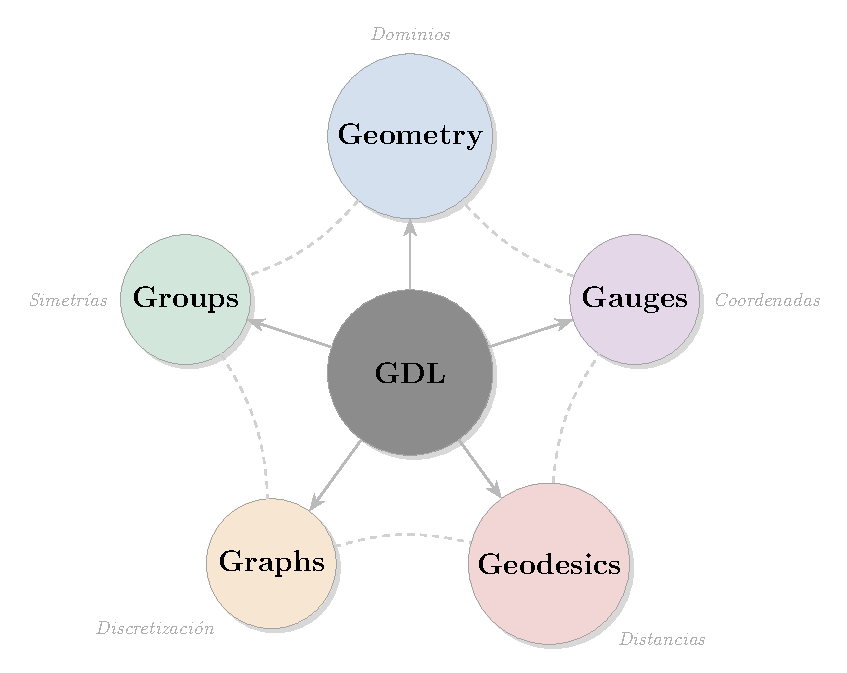
\includegraphics[width=0.7\textwidth]{images/five_gs_framework.pdf}
\caption[The five G's of Geometric Deep Learning]{The five fundamental G's of Geometric Deep Learning. Each component represents an essential aspect of the unifying framework: \textbf{Geometry} (domains), \textbf{Groups} (symmetries), \textbf{Graphs} (discretization), \textbf{Geodesics} (distances), and \textbf{Gauges} (local coordinates).}
\label{fig:five_gs_framework}
\end{figure}

\autoref{fig:jerarquia_5gs} complements this view by showing the hierarchical structure of the five G's, from the most fundamental base (the geometry of the domain) to the most specific levels of abstraction.

\begin{figure}[htbp]
\centering
\begin{tikzpicture}[scale=0.75]
% Definir estilos
\tikzset{
    level/.style={rectangle, rounded corners=3pt, draw, minimum width=2.8cm, minimum height=0.7cm, align=center, font=\small\bfseries},
    arrow/.style={->, thick, >=stealth, gray!70},
    desc/.style={font=\scriptsize, text=black!60, align=left}
}

% Niveles de la pirámide (de abajo hacia arriba)
\node[level, fill=gdlgreen!15, minimum width=10cm] (geom) at (0,0) {Geometry};
\node[level, fill=gdlgreen!25, minimum width=8cm] (grupos) at (0,1.2) {Groups};
\node[level, fill=gdlgreen!35, minimum width=6cm] (grafos) at (0,2.4) {Graphs};
\node[level, fill=gdlgreen!45, minimum width=4cm] (geod) at (0,3.6) {Geodesics};
\node[level, fill=gdlgreen!55, minimum width=2.5cm] (gauges) at (0,4.8) {Gauges};

% Flechas de relación
\draw[arrow] (geom.north) ++(0,0.1) -- ++(0,0.3);
\draw[arrow] (grupos.north) ++(0,0.1) -- ++(0,0.3);
\draw[arrow] (grafos.north) ++(0,0.1) -- ++(0,0.3);
\draw[arrow] (geod.north) ++(0,0.1) -- ++(0,0.3);

% Descripciones a la derecha (posiciones relativas al borde de cada nivel)
\node[desc, anchor=west] at (geom.east) {\quad Domain $\Omega$ where data live};
\node[desc, anchor=west] at (grupos.east) {\quad Symmetries $G$ that preserve structure};
\node[desc, anchor=west] at (grafos.east) {\quad Discretization of the domain};
\node[desc, anchor=west] at (geod.east) {\quad Information propagation};
\node[desc, anchor=west] at (gauges.east) {\quad Local invariances};

% Símbolos a la izquierda (posiciones relativas al borde de cada nivel)
\node[font=\scriptsize, anchor=east] at (geom.west) {$\mathbb{R}^n$, $\mathcal{M}$, $\mathcal{G}$\quad};
\node[font=\scriptsize, anchor=east] at (grupos.west) {$\text{SO}(n)$, $S_n$, $E(n)$\quad};
\node[font=\scriptsize, anchor=east] at (grafos.west) {$G=(V,E)$\quad};
\node[font=\scriptsize, anchor=east] at (geod.west) {$d(x,y)$, paths\quad};
\node[font=\scriptsize, anchor=east] at (gauges.west) {frames\quad};

\end{tikzpicture}
\caption[Hierarchy of the five G's of GDL]{Hierarchical structure of the five G's of Geometric Deep Learning. From the base, \textbf{Geometry} defines the domain where data reside; \textbf{Groups} capture the symmetries of the problem; \textbf{Graphs} discretize the domain; \textbf{Geodesics} determine how information propagates; and \textbf{Gauges} handle local invariances in coordinate systems.}
\label{fig:jerarquia_5gs}
\end{figure}

From this unifying perspective, \gls{GDL} establishes that effective processing of signals over geometric domains requires respecting three fundamental principles:

\begin{enumerate}
    \item \textbf{Geometric locality}: Operations must be local with respect to the metric of the domain. Geometric architectures exploit local structure through neighborhoods defined by the underlying geometry, allowing information to propagate consistently with the intrinsic distances of the space (see \autoref{sec:grafos_discretizacion} for the formalization through graphs).

    \item \textbf{Equivariance}: Transformations must preserve the relevant symmetries of the problem. An equivariant function commutes with the actions of the symmetry group, ensuring that equivalent transformations of the input produce corresponding transformations in the output (see Section~\ref{subsec:equivarianza_invarianza} for the complete theory).

    \item \textbf{Compositionality}: Complex representations are built hierarchically through composition of simpler operations. The composition of equivariant layers preserves equivariance end to end (\autoref{theorem:equivariant_composition}), enabling deep architectures that maintain the desired geometric properties. This property is fundamental to the Equivariant Universal Approximation Theorem (\autoref{theorem:universal_approximation_equivariant}), which guarantees the expressive power of equivariant networks.
\end{enumerate}

\section{Geometry: The Domains of Data}\label{sec:geometria_dominios}

To design effective neural architectures in \gls{GDL}, we must understand the \textbf{intrinsic geometry} of the domains (\autoref{def:dominio_datos}) where data reside. Different types of data naturally inhabit different geometric spaces, and recognizing and respecting these geometries is decisive for the success of Deep Learning. The formal concepts of symmetry and equivariance are developed in \autoref{sec:grupos_simetrias}.

The choice of the geometric domain is neither arbitrary nor merely technical: it reflects the intrinsic structure of the data and determines which operations are natural and efficient. While the Deep Learning tradition has favored standard vector representations (vectors, matrices, tensors in $\mathbb{R}^n$) in a Euclidean space, much real-world data possesses intrinsic geometries that these representations do not adequately capture. Molecules naturally live in spaces with symmetries of the Euclidean group $E(3)$, hierarchies are better represented in hyperbolic spaces $\mathbb{H}^n$, and omnidirectional directions inhabit spheres $S^n$. Forcing this data into Euclidean spaces destroys valuable structural information and hinders effective learning.

\subsection{Geometry of Data}\label{subsec:geometria_datos}

In \autoref{ch:neural_networks} we established the fundamental conceptual framework of signals over structured domains (see \autoref{sec:datos_estructura}), where we introduced the distinction between \textit{domain} ($\Omega$), \textit{structure} ($\mathcal{S}$), and \textit{signal} ($f$). This framework allowed us to formally characterize different types of data through the triple $(\Omega, \mathcal{S}, f)$ or, equivalently, through the geometry-attributes pair $(\mathcal{D}, f)$ where $\mathcal{D} = (\Omega, \mathcal{S})$ represents the geometry of the domain and $f$ the observed attributes.

The concept of \textit{geometry of data} deepens this perspective, referring to the natural geometric structures that emerge from the intrinsic nature of the data, beyond their superficial numerical representations. \gls{GDL} proposes that these intrinsic geometries $\mathcal{D} = (\Omega, \mathcal{S})$ are not merely representation details, but fundamental properties that determine which neural architectures are appropriate and effective for each type of data.

\paragraph{From Euclidean representations to complex geometric structures}

Traditionally, machine learning has operated under the paradigm that all data can be represented as:

\begin{itemize}
    \item \textbf{Vectors}: $\mathbb{R}^n$ (sequences, embeddings, extracted features)
    \item \textbf{Matrices}: $\mathbb{R}^{n \times m}$ (grayscale images, tabular data tables)
    \item \textbf{Higher-order tensors}: $\mathbb{R}^{n_1 \times n_2 \times \cdots \times n_k}$ (RGB images as $\mathbb{R}^{H \times W \times 3}$, video as $\mathbb{R}^{T \times H \times W \times 3}$)
\end{itemize}

This simplifying perspective has been tremendously successful. However, this view is fundamentally limited. Let us revisit some of the examples presented in \autoref{ch:neural_networks} to examine the limitations of Euclidean representations from the perspective of \gls{GDL}:

\begin{itemize}
    \item \textbf{Molecules as 3D graphs} (cf.~\autoref{ex:molecula}): A molecule is not simply a set of atomic coordinates in $\mathbb{R}^{3n}$. As we saw earlier, its structure combines \textit{discrete connectivity} (graph of covalent chemical bonds) with \textit{continuous three-dimensional geometry} (spatial positions of atoms). More fundamentally, the physicochemical properties are invariant under the Euclidean group $E(3)$ of translations, rotations, and reflections. Vectorizing the coordinates arbitrarily breaks these natural symmetries and forces neural networks to relearn fundamental physical invariances.

    \item \textbf{Social networks} (cf.~\autoref{ex:red_social}): A social graph $G = (V, E)$ lacks a natural ordering among its nodes. Assigning indices $\{1, 2, \ldots, n\}$ to users and attempting to represent the graph as an adjacency matrix $A \in \mathbb{R}^{n \times n}$ introduces a completely artificial ordering. The relevant structure is purely topological: who is connected to whom, not in which ``position'' each user is.

    \item \textbf{Physical surfaces} (cf.~\autoref{ex:superficie_riemanniana}): A 3D surface (the cerebral cortex, the surface of a protein, a scanned object) is naturally a 2D Riemannian manifold embedded in $\mathbb{R}^3$. The geodesic distances over the surface and the intrinsic curvature are fundamental geometric properties independent of how we parameterize or triangulate the surface. A triangular mesh with $n$ vertices is not simply a tensor $\mathbb{R}^{n \times 3}$ of coordinates: it is a discretization of an underlying continuous manifold.
\end{itemize}

These examples illustrate a fundamental principle: data possesses intrinsic geometries that standard vector representations do not fully capture. \gls{GDL} proposes a paradigm shift: instead of forcing all data into $\mathbb{R}^n$, we must design architectures that operate directly on the natural geometries of the data.

\subsection{Traditional Euclidean Geometry}\label{subsec:geometria_euclidiana}

In order to understand the differences between geometries we must first understand traditional Euclidean geometry. The Euclidean space $\mathbb{R}^n$ constitutes the most familiar and widely used geometric domain in classical Deep Learning. Its ubiquity is not accidental: the Euclidean structure provides computational simplicity, well-developed analytical tools, and uniform representations that have proven effective in many applications.

\paragraph{Euclid's postulates}

Euclidean geometry is grounded in the five postulates established by Euclid in his \textit{Elements} \citep{euclid1956elements}. These axioms define the fundamental properties of flat space:

\begin{enumerate}
    \item \textbf{Postulate of the line}: Through two distinct points passes exactly one line.
    \item \textbf{Postulate of the segment}: Every segment can be extended indefinitely into a straight line.
    \item \textbf{Postulate of the circle}: Given a point and a distance, a circle can be drawn with center at that point and radius equal to that distance.
    \item \textbf{Postulate of right angles}: All right angles are equal to one another.
    \item \textbf{Postulate of parallels}: Through a point external to a line, exactly one line parallel to the first passes.
\end{enumerate}

The fifth postulate, known as the \textit{parallel postulate} or \textit{Euclid's postulate}, is historically the most controversial. For more than two millennia, mathematicians attempted to derive it from the other four, until in the 19th century Gauss, Bolyai, and Lobachevsky independently demonstrated that negating it produces consistent geometries: the \textit{non-Euclidean geometries} \citep{gray2007worlds}.

\paragraph{Modern mathematical formalization}

Intuitively, \textit{Euclidean geometry} is that which uses the Euclidean metric, or $\ell^2$ norm, to measure distances

\[
d(\mathbf{x}, \mathbf{y}) = \|\mathbf{x} - \mathbf{y}\|_2 = \sqrt{\sum_{i=1}^n (x_i - y_i)^2}
\]

This metric defines notions of distance, neighborhood, and continuity that are uniform and well behaved: it satisfies the properties we expect of everyday ``flat'' space: shortest paths are straight lines, triangles have angles that sum to $\pi$, and parallel lines remain equidistant. Moreover, the fundamental operations (inner products, projections, convolutions) have efficient closed forms and well-understood analytical properties.

In the language of modern differential geometry, the Euclidean space $\mathbb{R}^n$ is a Riemannian manifold (\autoref{def:metrica_riemanniana} and \autoref{subsec:variedades_riemannianas}) with the following characteristic properties (the referenced concepts are developed formally later in this chapter):

\begin{itemize}
    \item \textbf{Flat Riemannian metric}: The Riemannian metric $g$ is constant and equal to the identity ($g_{ij} = \delta_{ij}$), which induces the standard Euclidean distance (see \autoref{subsec:variedades_riemannianas}).
    \item \textbf{Zero curvature}: The sectional curvature (\autoref{def:curvatura_preliminar}) is $K = 0$ at every point and direction.
    \item \textbf{Straight geodesics}: The geodesics (\autoref{def:geodesica}) are straight lines, formalizing Euclid's postulates 1 and 2.
    \item \textbf{Symmetry group}: The group of isometries is the \textit{Euclidean group} $E(n) = \mathbb{R}^n \rtimes O(n)$ (\autoref{def:grupo}, \autoref{def:producto_semidirecto}), which includes rotations, reflections, and translations combined through the semidirect product.
\end{itemize}

The deep connection between Euclid's classical geometry and modern differential geometry is established through the following fundamental result (see \autoref{sec:gauss_bonnet} of Appendix~\ref{ch:teoremas_complementarios} for the generalized theorem and its proof):

\begin{theorem}[Gauss-Bonnet for geodesic triangles]\label{thm:gauss_bonnet_triangulo}
Let $\mathcal{M}$ be a Riemannian surface with Gaussian curvature $K$, and let $T \subset \mathcal{M}$ be a geodesic triangle with interior angles $\alpha$, $\beta$, $\gamma$. Then:
\begin{equation}\label{eq:gauss_bonnet_triangulo}
\alpha + \beta + \gamma = \pi + \int_T K \, dA
\end{equation}
where $dA$ denotes the area element induced by the Riemannian metric.
\end{theorem}

This theorem \citep{lee2018introduction} has a fundamental consequence: when $K = 0$ (zero curvature), we recover the classical Euclidean result that the angles of a triangle sum to exactly $\pi$. Moreover, the theorem demonstrates that Euclid's fifth postulate (parallels) is \textit{equivalent} to the condition of Gaussian curvature $K = 0$.

\paragraph{Limitations of Euclidean geometry}

However, Euclidean geometry is not universal. When data has intrinsically non-Euclidean structure, forcing it into standard vector/matrix representations destroys important structural information:

\begin{itemize}
    \item \textbf{Spherical images} ($360^\circ$ panoramas): They naturally live on the sphere $S^2$, but the equirectangular projection to $\mathbb{R}^{H \times W}$ introduces extreme distortions at the poles. The $\ell^2$ distance between pixels does not respect the geodesic distances over $S^2$. Rotations in $SO(3)$ become complex and nonlinear transformations in the matrix representation.

    \item \textbf{3D point clouds} (cf.~\autoref{ex:nube_puntos}): Sets $\{p_1, \ldots, p_n\} \subset \mathbb{R}^3$ without a canonical ordering. Forcibly vectorizing them into $\mathbb{R}^{3n}$ imposes an arbitrary ordering that is not intrinsic to the geometric object, violating the natural permutation invariance.

    \item \textbf{Molecular structures}: They have complex three-dimensional geometry with symmetries of the Euclidean group $E(3)$. Representing them as vectors in $\mathbb{R}^d$ breaks the fundamental physical invariances under rotations and translations.

    \item \textbf{Hierarchical data}: They naturally live in hyperbolic spaces $\mathbb{H}^n$ where distance captures hierarchy. Embeddings in Euclidean $\mathbb{R}^n$ require exponentially higher dimensionality to preserve distances \citep{nickel2017poincare}.
\end{itemize}

\subsection{Foundations of Manifolds}\label{subsec:fundamentos_variedades}

To formalize the idea that data resides in spaces with intrinsic geometry, we need the mathematical concept of \textit{manifold}. This subsection develops the necessary foundations, beginning with topological preliminaries and progressing toward differentiable manifolds.

\subsubsection{Topological preliminaries}\label{subsubsec:preliminares_topologicos}

Before introducing the concept of manifold, we need to establish the necessary topological foundations. For a complete exposition of these concepts, see~\citet{munkres2000topology}.

\begin{definition}[Topological space]\label{def:espacio_topologico}
A \textit{topological space} is a pair $(X, \tau)$ where $X$ is a set and $\tau$ is a collection of subsets of $X$ (called \textbf{open sets}) that satisfies:
\begin{enumerate}
	\item $\emptyset, X \in \tau$ (the empty set and the whole set are open)
	\item The arbitrary union of open sets is open: if $\{U_\alpha\}_{\alpha \in I} \subset \tau$, then $\bigcup_{\alpha \in I} U_\alpha \in \tau$
	\item The finite intersection of open sets is open: if $U_1, \ldots, U_n \in \tau$, then $\bigcap_{i=1}^n U_i \in \tau$
\end{enumerate}
The collection $\tau$ is called a \textbf{topology} on $X$.
\end{definition}

\begin{definition}[Hausdorff space]\label{def:espacio_hausdorff}
A topological space $(X, \tau)$ is a \textit{Hausdorff space} (or $T_2$) if for any two distinct points $x, y \in X$ with $x \neq y$, there exist disjoint open sets $U, V \in \tau$ such that $x \in U$, $y \in V$ and $U \cap V = \emptyset$.

Intuitively, this means that points can be ``separated'' by open sets.
\end{definition}

\begin{definition}[Countable base]\label{def:base_numerable}
A topological space $(X, \tau)$ has a \textit{countable base} (or satisfies the second axiom of countability) if there exists a countable collection $\mathcal{B} = \{B_n\}_{n \in \mathbb{N}}$ of open sets such that every open set of $\tau$ can be expressed as a union of elements of $\mathcal{B}$.

Formally, $\mathcal{B} \subset \tau$ is a base if for every $U \in \tau$ and every $x \in U$, there exists $B \in \mathcal{B}$ such that $x \in B \subseteq U$.
\end{definition}

\begin{definition}[Homeomorphism]\label{def:homeomorfismo}
Let $(X, \tau_X)$ and $(Y, \tau_Y)$ be topological spaces. A function $f: X \to Y$ is a \textit{homeomorphism} if:
\begin{enumerate}
	\item $f$ is bijective
	\item $f$ is continuous: for every $V \in \tau_Y$, we have $f^{-1}(V) \in \tau_X$
	\item $f^{-1}$ is continuous: for every $U \in \tau_X$, we have $(f^{-1})^{-1}(U) = f(U) \in \tau_Y$
\end{enumerate}
Two spaces are \textit{homeomorphic} if there exists a homeomorphism between them. Intuitively, they are ``topologically identical''.
\end{definition}

\subsubsection{Topological manifolds}\label{subsubsec:variedades_topologicas}

With these concepts established, we can now rigorously define topological manifolds. For a complete development of manifold theory, we recommend~\citet{lee2012introduction}.

\begin{definition}[Topological manifold]\label{def:variedad_topologica}
A \textit{topological manifold} of dimension $m$ is a topological space $\mathcal{M}$ that satisfies:
\begin{enumerate}
	\item $\mathcal{M}$ is a Hausdorff space
	\item $\mathcal{M}$ has a countable base
	\item $\mathcal{M}$ is locally Euclidean of dimension $m$: for every point $p \in \mathcal{M}$, there exists an open neighborhood $U \ni p$ and a homeomorphism $\phi: U \to V$ where $V$ is an open set of $\mathbb{R}^m$
\end{enumerate}
\end{definition}

Intuitively, a manifold is a space that locally ``resembles'' Euclidean space, although globally it may have a very different structure. We can illustrate it with the following examples:

\begin{itemize}
    \item \textbf{The Earth as a 2D manifold}: Although we know the Earth is approximately spherical, when we walk through a city, we locally perceive the ground as flat. This is precisely the concept of a manifold: a space that can be globally curved, but locally behaves like the familiar Euclidean space.
    \item \textbf{A crumpled sheet of paper}: If we crumple a sheet, it remains locally two-dimensional (we can place a finger at any point and move it in two independent directions), but globally it has a complex shape in three-dimensional space.
    \item \textbf{The configuration space of a robot}: A robotic arm with multiple joints has a configuration space that is not Euclidean, but locally we can parameterize nearby positions with standard coordinates.
\end{itemize}

This intuition is crucial because many high-dimensional datasets (images, text, signals) actually ``live'' on manifolds of much lower dimension, and exploiting this significantly improves learning.

\begin{definition}[Atlas and charts]\label{def:atlas_cartas}
An \textit{atlas} of dimension $m$ for a topological space $\mathcal{M}$ is a collection $\mathcal{A} = \{(U_\alpha, \phi_\alpha)\}_{\alpha \in I}$ where:
\begin{itemize}
	\item $\{U_\alpha\}_{\alpha \in I}$ is an open cover of $\mathcal{M}$
	\item Each $\phi_\alpha: U_\alpha \to V_\alpha \subset \mathbb{R}^m$ is a homeomorphism (called a \textit{chart})
\end{itemize}

The transition functions $\phi_\beta \circ \phi_\alpha^{-1}: \phi_\alpha(U_\alpha \cap U_\beta) \to \phi_\beta(U_\alpha \cap U_\beta)$ determine the structure of the manifold.
\end{definition}

\begin{figure}[htbp]
\centering
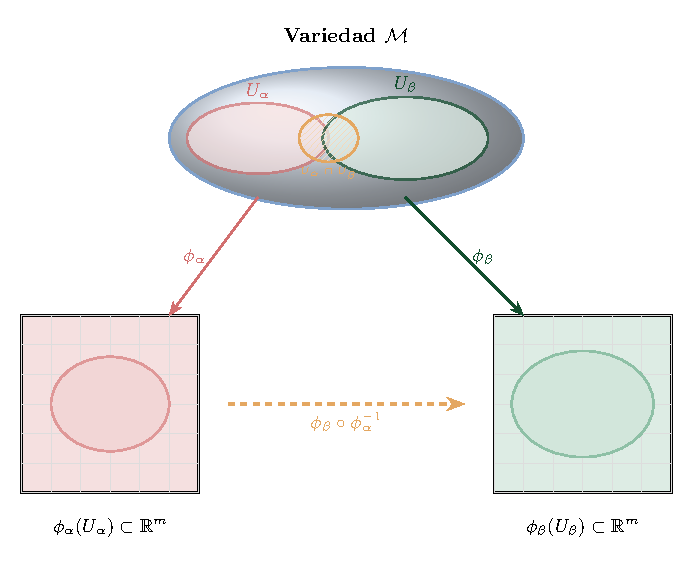
\includegraphics[width=0.75\textwidth]{images/charts_atlas.pdf}
\caption[Atlas and charts of a manifold]{Atlas $\mathcal{A} = \{(U_\alpha, \phi_\alpha)\}_{\alpha \in I}$ of a manifold $\mathcal{M}$: each chart $(U_\alpha, \phi_\alpha)$ is a homeomorphism $\phi_\alpha: U_\alpha \to V_\alpha \subset \mathbb{R}^m$ that defines local coordinates on an open set of $\mathcal{M}$. The transition function $\phi_\beta \circ \phi_\alpha^{-1}: \phi_\alpha(U_\alpha \cap U_\beta) \to \phi_\beta(U_\alpha \cap U_\beta)$ connects the representations of overlapping charts.}
\label{fig:charts_atlas}
\end{figure}

\subsubsection{Differentiable manifolds and tangent space}\label{subsubsec:variedades_diferenciables}

\begin{definition}[Smooth function]\label{def:funcion_suave}
Let $U \subseteq \mathbb{R}^n$ be an open set. A function $f: U \rightarrow \mathbb{R}^m$ is \textit{smooth} (or of \textit{class $C^\infty$}) if it possesses continuous partial derivatives of all orders.
\end{definition}

More generally, a function between differentiable manifolds is smooth if its expression in local coordinates is smooth.

\begin{definition}[Differentiable manifold]\label{def:variedad_diferenciable}
A topological manifold $\mathcal{M}$ is \textit{differentiable} (or smooth) if it possesses an atlas $\mathcal{A} = \{(U_\alpha, \phi_\alpha)\}$ such that all its transition maps $\phi_\beta \circ \phi_\alpha^{-1}$ are of class $C^\infty$.
\end{definition}

The differentiable structure allows defining concepts from calculus (derivatives, integrals, differential equations) on the manifold. The most fundamental concept is that of the \textit{tangent space}, which captures the notion of ``infinitesimal directions'' at each point. We present two equivalent constructions that offer complementary perspectives.

\begin{definition}[Tangent space via curves]\label{def:espacio_tangente_curvas}
Let $\mathcal{M}$ be a differentiable manifold and $p \in \mathcal{M}$. Two curves $\gamma_1, \gamma_2: (-\epsilon, \epsilon) \to \mathcal{M}$ with $\gamma_1(0) = \gamma_2(0) = p$ are said to be \textit{tangent at $p$} if for some (and therefore every) chart $(U, \phi)$ with $p \in U$:
\[
\frac{d}{dt}\bigg|_{t=0} (\phi \circ \gamma_1)(t) = \frac{d}{dt}\bigg|_{t=0} (\phi \circ \gamma_2)(t)
\]
The \textit{tangent space} $T_p\mathcal{M}$ is the set of equivalence classes $[\gamma]$ of curves tangent at $p$.
\end{definition}

This definition captures the geometric intuition: a tangent vector represents a ``direction of motion'' from the point $p$, determined by the initial velocity of any curve passing through $p$ in that direction.

\begin{remark}[Vector space structure]\label{rem:estructura_vectorial_curvas}
The set $T_p^{\text{curvas}}\mathcal{M}$ admits a vector space structure induced by any chart $(U, \phi)$ with $p \in U$. The map $[\gamma] \mapsto (\phi \circ \gamma)'(0) \in \mathbb{R}^m$ is a bijection between $T_p^{\text{curvas}}\mathcal{M}$ and $\mathbb{R}^m$, and we \textit{transport} the vector structure of $\mathbb{R}^m$ to $T_p^{\text{curvas}}\mathcal{M}$ through this bijection. That is, we define:
\[
\alpha[\gamma_1] + [\gamma_2] \;=\; \bigl[\gamma\bigr], \quad \text{where $(\phi \circ \gamma)'(0) = \alpha(\phi \circ \gamma_1)'(0) + (\phi \circ \gamma_2)'(0)$}.
\]
This structure is \textit{independent of the chosen chart}: if $(V, \psi)$ is another chart with $p \in V$, the chain rule applied to the transition function $\psi \circ \phi^{-1}$ guarantees that the isomorphism induced by $\psi$ is compatible with the one induced by $\phi$.
\end{remark}

\begin{definition}[Tangent space via derivations]\label{def:espacio_tangente_derivaciones}
Let $\mathcal{M}$ be a differentiable manifold and $p \in \mathcal{M}$. A \textit{derivation at $p$} is a linear map $v: C^\infty(\mathcal{M}) \to \mathbb{R}$ that satisfies the Leibniz rule for all $f, g \in C^\infty(\mathcal{M})$:
\[
v(fg) = v(f)g(p) + f(p)v(g)
\]
The \textit{tangent space} $T_p\mathcal{M}$ is the vector space of all derivations at $p$.
\end{definition}

This algebraic definition captures the idea that a tangent vector is a ``directional derivative operator'': given a vector $v$ and a function $f$, $v(f)$ represents the rate of change of $f$ in the direction $v$.

\begin{lemma}[Decomposition of derivations in coordinates]\label{lem:descomposicion_derivaciones}
Let $\mathcal{M}$ be a differentiable manifold of dimension $m$, $p \in \mathcal{M}$ and $(U, \phi)$ a chart with $\phi(p) = 0$ and coordinate functions $x^1, \ldots, x^m$. Then:
\begin{enumerate}
	\item Derivations are local operators: if $f = g$ in a neighborhood of $p$, then $v(f) = v(g)$ for every derivation $v$ at $p$. This allows evaluating $v$ on functions defined only on $U$, extending them to $\mathcal{M}$ through bump functions, with a result independent of the extension.
	\item Every derivation $v$ at $p$ is expressed as:
	\[
	v = \sum_{j=1}^{m} v(x^j) \frac{\partial}{\partial x^j}\bigg|_p
	\]
	where $\frac{\partial}{\partial x^j}\big|_p(f) = \frac{\partial(f \circ \phi^{-1})}{\partial x^j}\big|_{\phi(p)}$. In particular, $\dim T_p^{\text{deriv}}\mathcal{M} = m$.
\end{enumerate}
\end{lemma}

\begin{proof}
\textbf{(1) Locality.} Let $\chi \in C^\infty(\mathcal{M})$ be a bump function with $\chi \equiv 1$ in a neighborhood $W \subset U$ of $p$ and $\operatorname{supp}(\chi) \subset U$. If $f = g$ in $U$, then $\chi(f - g) = 0$ on all of $\mathcal{M}$. By the Leibniz rule, $0 = v(\chi(f-g)) = v(\chi)(f-g)(p) + \chi(p) \, v(f-g) = v(f-g)$, since $\chi(p) = 1$ and $(f-g)(p) = 0$.

\textbf{(2) Decomposition.} First, every derivation annihilates constants: if $c \in \mathbb{R}$, then $v(c) = v(c \cdot 1) = c \, v(1)$ and $v(1) = v(1 \cdot 1) = v(1) \cdot 1 + 1 \cdot v(1) = 2v(1)$, whence $v(1) = 0$ and therefore $v(c) = 0$.

Let $f \in C^\infty(\mathcal{M})$. We write $\hat{f} = f \circ \phi^{-1}: \phi(U) \to \mathbb{R}$. By the fundamental theorem of calculus with integral remainder, for $\mathbf{x} = (x^1, \ldots, x^m)$ in a convex neighborhood of $0 \in \phi(U)$:
\[
\hat{f}(\mathbf{x}) = \hat{f}(0) + \sum_{j=1}^{m} x^j \, g_j(\mathbf{x}), \quad \text{where } g_j(\mathbf{x}) = \int_0^1 \frac{\partial \hat{f}}{\partial x^j}(t\mathbf{x}) \, dt
\]
The functions $g_j$ are smooth and $g_j(0) = \frac{\partial \hat{f}}{\partial x^j}(0)$. Composing with $\phi$ and using locality (item 1), we obtain on $U$:
\[
f = f(p) + \sum_{j=1}^{m} x^j \cdot (g_j \circ \phi)
\]
where we identify $x^j$ with the coordinate function $x^j = \pi^j \circ \phi$. Applying $v$ and using that $v$ annihilates constants, $x^j(p) = 0$ and the Leibniz rule:
\[
v(f) = \sum_{j=1}^{m} \bigl[v(x^j) \cdot g_j(\phi(p)) + x^j(p) \cdot v(g_j \circ \phi)\bigr] = \sum_{j=1}^{m} v(x^j) \frac{\partial(f \circ \phi^{-1})}{\partial x^j}\bigg|_{0}
\]
This shows that $v = \sum_j v(x^j) \frac{\partial}{\partial x^j}\big|_p$. Since $\frac{\partial}{\partial x^j}\big|_p(x^k) = \delta_j^k$, the derivations $\{\frac{\partial}{\partial x^j}\big|_p\}_{j=1}^m$ are linearly independent and generate $T_p^{\text{deriv}}\mathcal{M}$ \citep[Proposition 3.2]{lee2012introduction}.
\end{proof}

\begin{proposition}[Equivalence of the definitions of tangent space]\label{prop:equivalencia_espacio_tangente}
The two definitions of tangent space are canonically isomorphic (the isomorphism is independent of the choice of coordinates). The isomorphism $\Phi: T_p^{\text{curvas}}\mathcal{M} \to T_p^{\text{deriv}}\mathcal{M}$ is given by:
\[
\Phi([\gamma])(f) = \frac{d}{dt}\bigg|_{t=0} (f \circ \gamma)(t)
\]
for every function $f \in C^\infty(\mathcal{M})$.
\end{proposition}

\begin{proof}
We proceed in four steps: we verify that $\Phi$ is well defined, that its image consists of derivations, and that it is bijective.

\textbf{Step 1: $\Phi$ is well defined.} Let $\gamma_1, \gamma_2$ be two curves with $\gamma_1(0) = \gamma_2(0) = p$ and $\gamma_1 \sim \gamma_2$ (that is, they are tangent at $p$). We must show that $\Phi([\gamma_1]) = \Phi([\gamma_2])$. Let $(U, \phi)$ be a local chart at $p$ with $\phi = (x^1, \ldots, x^m)$. By the definition of tangency, $(\phi \circ \gamma_1)'(0) = (\phi \circ \gamma_2)'(0)$. For any $f \in C^\infty(\mathcal{M})$, we factor $f \circ \gamma_i = (f \circ \phi^{-1}) \circ (\phi \circ \gamma_i)$ and apply the chain rule:
\[
(f \circ \gamma_i)'(0) = \sum_{j=1}^{m} \frac{\partial (f \circ \phi^{-1})}{\partial x^j}\bigg|_{\phi(p)} \cdot (x^j \circ \gamma_i)'(0)
\]
Since $(x^j \circ \gamma_i)'(0)$ is the $j$-th component of $(\phi \circ \gamma_i)'(0)$ and $(\phi \circ \gamma_1)'(0) = (\phi \circ \gamma_2)'(0)$, we conclude that $(f \circ \gamma_1)'(0) = (f \circ \gamma_2)'(0)$.

\textbf{Step 2: $\Phi([\gamma])$ is a derivation.} Let $v_\gamma = \Phi([\gamma])$. We verify the two properties:
\begin{itemize}
    \item \textit{Linearity}: For $f, g \in C^\infty(\mathcal{M})$ and $\alpha, \beta \in \mathbb{R}$:
    \begin{align*}
    v_\gamma(\alpha f + \beta g) &= \frac{d}{dt}\bigg|_{t=0} (\alpha f + \beta g)(\gamma(t)) \\
    &= \alpha \frac{d}{dt}\bigg|_{t=0} f(\gamma(t)) + \beta \frac{d}{dt}\bigg|_{t=0} g(\gamma(t)) = \alpha v_\gamma(f) + \beta v_\gamma(g)
    \end{align*}
    \item \textit{Leibniz rule}: For $f, g \in C^\infty(\mathcal{M})$, we apply the product rule for real functions of a real variable $t \mapsto f(\gamma(t))$ and $t \mapsto g(\gamma(t))$:
    \begin{align*}
    v_\gamma(fg) &= \frac{d}{dt}\bigg|_{t=0} \bigl[f(\gamma(t)) \cdot g(\gamma(t))\bigr] \\
    &= \left(\frac{d}{dt}\bigg|_{t=0} f(\gamma(t))\right) g(\gamma(0)) + f(\gamma(0)) \left(\frac{d}{dt}\bigg|_{t=0} g(\gamma(t))\right) \\
    &= v_\gamma(f) \, g(p) + f(p) \, v_\gamma(g)
    \end{align*}
\end{itemize}

\textbf{Step 3: $\Phi$ is injective.} Suppose that $\Phi([\gamma_1]) = \Phi([\gamma_2])$, that is, that for every $f \in C^\infty(\mathcal{M})$ we have $(f \circ \gamma_1)'(0) = (f \circ \gamma_2)'(0)$. Let $(U, \phi)$ be a chart with $p \in U$ and coordinate functions $x^j = \pi^j \circ \phi$, where $\pi^j: \mathbb{R}^m \to \mathbb{R}$ is the $j$-th projection. The functions $x^j$ are defined on $U$, but by the locality of $\Phi([\gamma])$ (see \autoref{lem:descomposicion_derivaciones}), we can evaluate them. Taking $f = x^j$, we obtain $(x^j \circ \gamma_1)'(0) = (x^j \circ \gamma_2)'(0)$ for all $j = 1, \ldots, m$. This implies $(\phi \circ \gamma_1)'(0) = (\phi \circ \gamma_2)'(0)$, that is, $\gamma_1 \sim \gamma_2$.

\textbf{Step 4: $\Phi$ is surjective.} Let $v \in T_p^{\text{deriv}}\mathcal{M}$ be an arbitrary derivation. Let $(U, \phi)$ be a chart with $\phi(p) = 0$ and coordinate functions $x^1, \ldots, x^m$. We define the vector $\mathbf{a} = (a^1, \ldots, a^m) \in \mathbb{R}^m$ by $a^j = v(x^j)$ and consider the curve $\gamma(t) = \phi^{-1}(t\mathbf{a}) = \phi^{-1}(ta^1, \ldots, ta^m)$. Then $\gamma(0) = \phi^{-1}(0) = p$ and for any $f \in C^\infty(\mathcal{M})$, the chain rule gives:
\[
\Phi([\gamma])(f) = \frac{d}{dt}\bigg|_{t=0} (f \circ \phi^{-1})(t\mathbf{a}) = \sum_{j=1}^{m} a^j \frac{\partial (f \circ \phi^{-1})}{\partial x^j}\bigg|_{0} = \sum_{j=1}^{m} v(x^j) \frac{\partial}{\partial x^j}\bigg|_p (f)
\]
By \autoref{lem:descomposicion_derivaciones}, $v = \sum_{j=1}^{m} v(x^j) \frac{\partial}{\partial x^j}\big|_p$, whence $\Phi([\gamma]) = v$.
\end{proof}

\textbf{Intuition about the two constructions.} The two constructions offer complementary perspectives:
\begin{itemize}
	\item \textbf{Curves}: They capture the geometric idea of ``directions of motion''. They are intuitive for visualizing tangent vectors as velocities of particles moving over the manifold.
	\item \textbf{Derivations}: They capture the analytical idea of ``directions of change of functions''. They are convenient for computations and generalize naturally to more abstract spaces.
\end{itemize}
In practice, we use both as convenient: curves for geometric intuition, derivations for algebraic manipulations.

\begin{example}[Tangent space to the sphere]\label{ex:espacio_tangente_esfera}
Consider the sphere $S^2 = \{(x,y,z) \in \mathbb{R}^3 : x^2 + y^2 + z^2 = 1\}$. At the north pole $p = (0,0,1)$:
\begin{itemize}
	\item \textbf{Via curves}: A tangent vector is the initial velocity of any curve over $S^2$ passing through $p$. For example, $\gamma(t) = (\sin t, 0, \cos t)$ has $\gamma(0) = p$ and $\gamma'(0) = (1, 0, 0)$.
	\item \textbf{Via derivations}: In stereographic coordinates $(u,v)$ centered at $p$, the derivations $\partial/\partial u$ and $\partial/\partial v$ form a basis.
\end{itemize}
The tangent space $T_p S^2$ is the plane $\{(x,y,0) : x,y \in \mathbb{R}\}$, which is horizontal and tangent to the sphere at the north pole.
\end{example}

\begin{figure}[htbp]
\centering
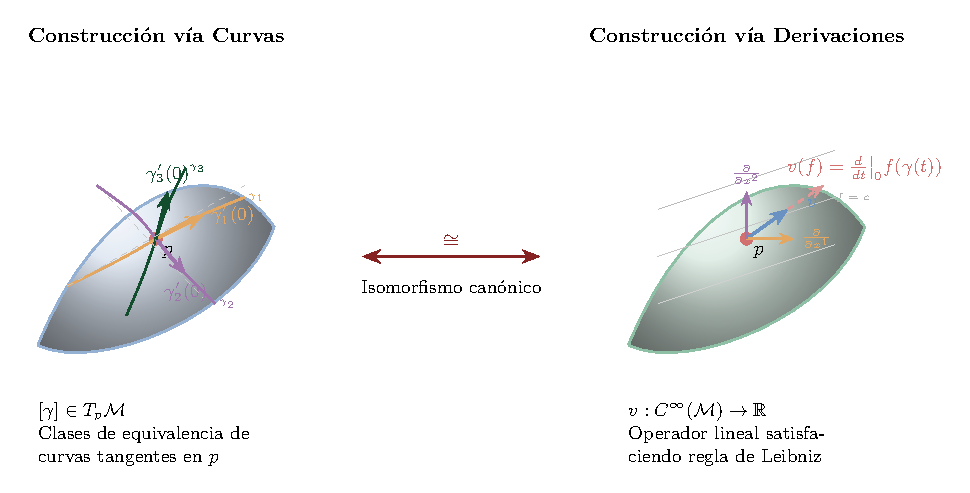
\includegraphics[width=0.7\textwidth]{images/tangent_space.pdf}
\caption[Tangent space to a manifold]{Tangent space $T_p\mathcal{M}$ at a point $p$ of a manifold. The tangent vectors represent initial velocities of curves passing through $p$, forming a vector space that linearly approximates the manifold at each point.}
\label{fig:tangent_space}
\end{figure}

\begin{definition}[Differential of a smooth map]\label{def:diferencial_aplicacion_suave}
Let $F: \mathcal{M} \to \mathcal{N}$ be a smooth map between differentiable manifolds. For each $p \in \mathcal{M}$, the \textit{differential} (or \textit{pushforward}) of $F$ at $p$ is the linear map $dF_p: T_p\mathcal{M} \to T_{F(p)}\mathcal{N}$ defined, in the formulation via derivations (\autoref{def:espacio_tangente_derivaciones}), by:
\[
dF_p(v)(g) = v(g \circ F) \quad \text{for all } g \in C^\infty(\mathcal{N}).
\]
If $(U, \phi)$ and $(V, \psi)$ are local charts at $p$ and $F(p)$ respectively, the expression of $dF_p$ in coordinates is the Jacobian matrix $\left(\frac{\partial (\psi \circ F \circ \phi^{-1})^i}{\partial x^j}\right)_{i,j}$.
\end{definition}

\begin{definition}[Smooth immersion]\label{def:inmersion_suave}
A smooth map $F: \mathcal{M} \to \mathcal{N}$ is an \textit{immersion} if its differential $dF_p: T_p\mathcal{M} \to T_{F(p)}\mathcal{N}$ is injective for every $p \in \mathcal{M}$. Equivalently, $\operatorname{rango}(dF_p) = \dim \mathcal{M}$ at each point.
\end{definition}

\begin{definition}[Smooth submersion]\label{def:submersion_suave}
A smooth map $F: \mathcal{M} \to \mathcal{N}$ is a \textit{submersion} if its differential $dF_p: T_p\mathcal{M} \to T_{F(p)}\mathcal{N}$ is surjective for every $p \in \mathcal{M}$. Equivalently, $\operatorname{rango}(dF_p) = \dim \mathcal{N}$ at each point, which requires $\dim \mathcal{M} \geq \dim \mathcal{N}$.
\end{definition}

\begin{remark}\label{rem:inmersion_submersion_dualidad}
Immersion and submersion are dual notions: the former requires $dF_p$ to be injective ($\operatorname{rango} = \dim \mathcal{M}$, needing $\dim \mathcal{M} \leq \dim \mathcal{N}$), while the latter requires surjectivity ($\operatorname{rango} = \dim \mathcal{N}$, needing $\dim \mathcal{M} \geq \dim \mathcal{N}$). The Regular Level Set Theorem (\autoref{thm:nivel_regular} of \autoref{ch:teoremas_complementarios}) guarantees that, if $F$ is a submersion, each fiber $F^{-1}(q)$ is a smooth submanifold of $\mathcal{M}$ of dimension $\dim \mathcal{M} - \dim \mathcal{N}$. This property of fibers as submanifolds will be fundamental in the theory of principal bundles (\autoref{subsec:fibrados_principales}), where the projection $\pi: P \to \mathcal{M}$ is a smooth submersion.
\end{remark}

\begin{definition}[Smooth embedding]\label{def:embebimiento_suave}
An \textit{immersion} $F: \mathcal{M} \to \mathcal{N}$ is an \textit{embedding} if in addition it is injective and is a homeomorphism onto its image $F(\mathcal{M})$ with the subspace topology.
\end{definition}

\begin{remark}\label{rem:compacta_inmersion_embebimiento}
If $\mathcal{M}$ is compact, every injective immersion $F: \mathcal{M} \to \mathcal{N}$ is automatically an embedding. Indeed, $F$ is a continuous, injective, and closed function (every continuous map from a compact space into a Hausdorff space is closed), whence $F$ is a homeomorphism onto its image.
\end{remark}

\subsubsection{Cotangent space and differential forms}\label{subsubsec:espacio_cotangente}

The tangent space $T_p\mathcal{M}$ captures the \textit{directions} at a point of the manifold; its dual, the \textit{cotangent space}, captures how \textit{functions change} along those directions. This step from vectors to covectors is essential for the differential geometry that underlies \gls{GDL}: the Riemannian metric (\autoref{subsec:variedades_riemannianas}), connections on bundles (\autoref{subsec:conexiones_fibrados}), and curvature (\autoref{def:curvatura_formal}) are expressed in terms of differential forms.

\begin{definition}[Cotangent space]\label{def:espacio_cotangente}
Let $\mathcal{M}$ be a differentiable manifold of dimension $m$ and $p \in \mathcal{M}$. The \textit{cotangent space} of $\mathcal{M}$ at $p$ is the algebraic dual of the tangent space:
\[
T_p^*\mathcal{M} = (T_p\mathcal{M})^* = \{\alpha: T_p\mathcal{M} \to \mathbb{R} \mid \alpha \text{ is linear}\}.
\]
The elements of $T_p^*\mathcal{M}$ are called \textit{covectors} (or \textit{pointwise 1-forms}). Since $\dim T_p\mathcal{M} = m$, we have $\dim T_p^*\mathcal{M} = m$.
\end{definition}

\begin{definition}[Differential of a function]\label{def:diferencial_funcion}
Let $f \in C^\infty(\mathcal{M})$ be a smooth function. The \textit{differential} of $f$ at $p$ is the covector $(df)_p \in T_p^*\mathcal{M}$ defined by:
\[
(df)_p(v) = v(f) \quad \text{for all } v \in T_p\mathcal{M},
\]
where $v(f)$ denotes the derivation $v$ applied to $f$ (\autoref{def:espacio_tangente_derivaciones}). In local coordinates $(x^1, \ldots, x^m)$, the differential is expressed as:
\[
df = \sum_{i=1}^m \frac{\partial f}{\partial x^i} \, dx^i.
\]
The covectors $\{dx^1, \ldots, dx^m\}$ form the \textit{dual basis} of $T_p^*\mathcal{M}$, determined by the duality relation with the basis $\{\partial/\partial x^j\}$ of $T_p\mathcal{M}$:
\[
dx^i\!\left(\frac{\partial}{\partial x^j}\right) = \delta^i_j.
\]
\end{definition}

\begin{remark}\label{rem:notacion_base_dual}
The notation $dx^i$ does not denote an ``infinitesimal'', but a well-defined linear functional: the covector that extracts the $i$-th component of a tangent vector with respect to the chart $(x^1, \ldots, x^m)$. This functional is precisely the differential of the coordinate function $x^i: \mathcal{M} \supset U \to \mathbb{R}$.
\end{remark}

\begin{definition}[Tensor product of covectors]\label{def:producto_tensorial_covectores}
Given $\alpha, \beta \in T_p^*\mathcal{M}$, their \textit{tensor product} is the bilinear form $\alpha \otimes \beta: T_p\mathcal{M} \times T_p\mathcal{M} \to \mathbb{R}$ defined by:
\[
(\alpha \otimes \beta)(v, w) = \alpha(v) \cdot \beta(w).
\]
The products $\{dx^i \otimes dx^j\}_{1 \leq i,j \leq m}$ form a basis of the space of $(0,2)$ tensors at $p$. In particular, the Riemannian metric (\autoref{def:metrica_riemanniana}) is expressed as $g_p = \sum_{i,j} g_{ij}(p) \, dx^i \otimes dx^j$.
\end{definition}

\begin{definition}[Differential 1-form]\label{def:1_forma_diferencial}
A \textit{differential 1-form} (or \textit{covector field}) on $\mathcal{M}$ is a smooth assignment $\omega: p \mapsto \omega_p \in T_p^*\mathcal{M}$. In local coordinates it is written $\omega = \sum_{i=1}^m \omega_i(x) \, dx^i$ with $\omega_i \in C^\infty(U)$. The space of all differential 1-forms is denoted $\Omega^1(\mathcal{M})$. Connections on principal bundles (\autoref{def:conexion_fibrado}) are 1-forms with values in a Lie algebra.
\end{definition}

\begin{definition}[Exterior product and $k$-forms]\label{def:producto_exterior_k_formas}
A \textit{differential $k$-form} on $\mathcal{M}$ is a smooth assignment that associates to each $p \in \mathcal{M}$ an antisymmetric tensor of type $(0, k)$. The space of $k$-forms is denoted $\Omega^k(\mathcal{M})$, with $\Omega^0(\mathcal{M}) = C^\infty(\mathcal{M})$ and $\Omega^k(\mathcal{M}) = 0$ for $k > m = \dim \mathcal{M}$; the 1-forms of \autoref{def:1_forma_diferencial} correspond to $k = 1$.

The \textit{exterior product} (or \textit{wedge}) is the operation
\[
\wedge: \Omega^k(\mathcal{M}) \times \Omega^l(\mathcal{M}) \longrightarrow \Omega^{k+l}(\mathcal{M})
\]
defined through the \textit{alternation operator} $\operatorname{Alt}$, which to a tensor $T$ of type $(0,n)$ assigns its totally antisymmetric part:
\[
\operatorname{Alt}(T)(v_1, \ldots, v_n) = \frac{1}{n!} \sum_{\sigma \in S_n} \operatorname{sgn}(\sigma)\, T(v_{\sigma(1)}, \ldots, v_{\sigma(n)}),
\]
where $S_n$ is the permutation group and $\operatorname{sgn}(\sigma) \in \{+1, -1\}$ the sign of~$\sigma$. The exterior product is defined as the normalized antisymmetrization of the tensor product (\autoref{def:producto_tensorial_covectores}):
\begin{equation}\label{eq:wedge_alt}
\alpha \wedge \beta = \frac{(k+l)!}{k!\,l!}\, \operatorname{Alt}(\alpha \otimes \beta),
\end{equation}
where $(\alpha \otimes \beta)(v_1, \ldots, v_{k+l}) = \alpha(v_1, \ldots, v_k)\,\beta(v_{k+1}, \ldots, v_{k+l})$. For 1-forms $\alpha, \beta \in \Omega^1(\mathcal{M})$, equation~\eqref{eq:wedge_alt} reduces to:
\[
(\alpha \wedge \beta)(v, w) = \alpha(v)\beta(w) - \alpha(w)\beta(v),
\]
which is equivalent to $\alpha \wedge \beta = \alpha \otimes \beta - \beta \otimes \alpha$. In particular, on the dual basis:
\[
dx^i \wedge dx^j = -dx^j \wedge dx^i, \qquad dx^i \wedge dx^i = 0.
\]
In general, the exterior product satisfies \textit{graded anticommutativity}: for $\alpha \in \Omega^k(\mathcal{M})$ and $\beta \in \Omega^l(\mathcal{M})$,
\[
\alpha \wedge \beta = (-1)^{kl}\, \beta \wedge \alpha.
\]
In local coordinates, every $k$-form is written:
\[
\omega = \sum_{i_1 < \cdots < i_k} \omega_{i_1 \cdots i_k}(x) \, dx^{i_1} \wedge \cdots \wedge dx^{i_k}.
\]
The volume element (\autoref{def:elemento_volumen}) is an $m$-form.
\end{definition}

\begin{proposition}[Algebraic properties of the exterior product]\label{prop:propiedades_producto_exterior}
The exterior product $\wedge$ satisfies the following properties for $\alpha \in \Omega^k(\mathcal{M})$, $\beta \in \Omega^l(\mathcal{M})$, $\gamma \in \Omega^r(\mathcal{M})$ and $f \in C^\infty(\mathcal{M})$:
\begin{enumerate}
    \item \textbf{Bilinearity}: $(\alpha + \alpha') \wedge \beta = \alpha \wedge \beta + \alpha' \wedge \beta$ and $\alpha \wedge (\beta + \beta') = \alpha \wedge \beta + \alpha \wedge \beta'$.
    \item \textbf{Associativity}: $(\alpha \wedge \beta) \wedge \gamma = \alpha \wedge (\beta \wedge \gamma)$.
    \item \textbf{Compatibility with scalars}: $(f\alpha) \wedge \beta = f(\alpha \wedge \beta) = \alpha \wedge (f\beta)$.
    \item \textbf{Graded anticommutativity}: $\alpha \wedge \beta = (-1)^{kl}\, \beta \wedge \alpha$.
\end{enumerate}
\end{proposition}

\begin{proof}
All the properties derive from definition~\eqref{eq:wedge_alt}: $\alpha \wedge \beta = \frac{(k+l)!}{k!\,l!}\, \operatorname{Alt}(\alpha \otimes \beta)$.

\textbf{(1) Bilinearity.} The tensor product $\otimes$ is bilinear and $\operatorname{Alt}$ is linear (being a linear combination of evaluations with fixed coefficients $\operatorname{sgn}(\sigma)/n!$). The composition~\eqref{eq:wedge_alt} preserves bilinearity.

\textbf{(3) Compatibility with scalars.} For $f \in C^\infty(\mathcal{M})$, we have $(f\alpha) \otimes \beta = f(\alpha \otimes \beta)$ pointwise, since $f(p)$ is a scalar that does not depend on the tangent vectors permuted by $\operatorname{Alt}$. By the linearity of $\operatorname{Alt}$:
\[
(f\alpha) \wedge \beta = \tfrac{(k+l)!}{k!\,l!}\,\operatorname{Alt}((f\alpha) \otimes \beta) = \tfrac{(k+l)!}{k!\,l!}\,f\cdot\operatorname{Alt}(\alpha \otimes \beta) = f(\alpha \wedge \beta).
\]
Analogously, $\alpha \wedge (f\beta) = f(\alpha \wedge \beta)$.

\textbf{(4) Graded anticommutativity.} Let $\tau \in S_{k+l}$ be the permutation $(1, \ldots, k+l) \mapsto (k{+}1, \ldots, k{+}l, 1, \ldots, k)$ that swaps the first $k$ indices with the last $l$. This permutation decomposes into $kl$ transpositions (each of the first $k$ elements crosses the last $l$), so $\operatorname{sgn}(\tau) = (-1)^{kl}$. The relation between the tensor products is:
\[
(\beta \otimes \alpha)(v_1, \ldots, v_{k+l}) = \beta(v_1, \ldots, v_l)\,\alpha(v_{l+1}, \ldots, v_{l+k}) = (\alpha \otimes \beta)(v_{\tau(1)}, \ldots, v_{\tau(k+l)}).
\]
Substituting into $\operatorname{Alt}$ and making the change $\rho = \tau \circ \sigma$ (which ranges over $S_{k+l}$ as $\sigma$ varies):
\begin{align*}
\operatorname{Alt}(\beta \otimes \alpha)(v_1, \ldots, v_{k+l})
  &= \frac{1}{(k{+}l)!}\sum_{\sigma \in S_{k+l}} \operatorname{sgn}(\sigma)\,(\alpha \otimes \beta)(v_{\tau\sigma(1)}, \ldots, v_{\tau\sigma(k+l)}) \\
  &= \frac{(-1)^{kl}}{(k{+}l)!}\sum_{\rho \in S_{k+l}} \operatorname{sgn}(\rho)\,(\alpha \otimes \beta)(v_{\rho(1)}, \ldots, v_{\rho(k+l)})
  = (-1)^{kl}\,\operatorname{Alt}(\alpha \otimes \beta),
\end{align*}
where we have used $\operatorname{sgn}(\tau\sigma) = (-1)^{kl}\operatorname{sgn}(\sigma)$. Multiplying by $\frac{(k+l)!}{k!\,l!}$ we obtain $\beta \wedge \alpha = (-1)^{kl}\,\alpha \wedge \beta$.

\textbf{(2) Associativity.} Let $n = k+l+r$. By~\eqref{eq:wedge_alt}:
\[
(\alpha \wedge \beta) \wedge \gamma = \frac{n!}{(k{+}l)!\,r!}\,\operatorname{Alt}_n\!\big((\alpha \wedge \beta) \otimes \gamma\big) = \frac{n!}{k!\,l!\,r!}\,\operatorname{Alt}_n\!\big(\operatorname{Alt}_{k+l}(\alpha \otimes \beta) \otimes \gamma\big).
\]
We identify $S_{k+l}$ with the subgroup of $S_n$ that fixes the last $r$ indices. For $\tau$ in this subgroup, $\tau$ acts only on the first $k+l$ arguments of $\alpha \otimes \beta$ and leaves $\gamma$ invariant. Evaluating explicitly:
\begin{align*}
&\operatorname{Alt}_n\!\big(\operatorname{Alt}_{k+l}(\alpha \otimes \beta) \otimes \gamma\big)(v_1, \ldots, v_n) \\
  &\quad= \frac{1}{n!\,(k{+}l)!}\sum_{\sigma \in S_n}\sum_{\tau \in S_{k+l}}\operatorname{sgn}(\sigma)\,\operatorname{sgn}(\tau)\,(\alpha \otimes \beta \otimes \gamma)(v_{\sigma(\tau(1))}, \ldots, v_{\sigma(\tau(n))}).
\end{align*}
Substituting $\rho = \sigma \circ \tau$: for each $\rho \in S_n$, the equation $\sigma \circ \tau = \rho$ with $\tau \in S_{k+l}$ admits exactly $(k{+}l)!$ solutions (since $\sigma = \rho \circ \tau^{-1}$ is determined). Since $\operatorname{sgn}(\sigma)\operatorname{sgn}(\tau) = \operatorname{sgn}(\rho)$:
\[
= \frac{(k{+}l)!}{n!\,(k{+}l)!}\sum_{\rho \in S_n}\operatorname{sgn}(\rho)\,(\alpha \otimes \beta \otimes \gamma)(v_{\rho(1)}, \ldots, v_{\rho(n)}) = \operatorname{Alt}_n(\alpha \otimes \beta \otimes \gamma).
\]
Therefore, $(\alpha \wedge \beta) \wedge \gamma = \frac{n!}{k!\,l!\,r!}\,\operatorname{Alt}_n(\alpha \otimes \beta \otimes \gamma)$. The computation for $\alpha \wedge (\beta \wedge \gamma)$ is identical, using $S_{l+r} \hookrightarrow S_n$ in the last positions, and produces the same expression.
\end{proof}

\begin{definition}[Exterior derivative]\label{def:derivada_exterior}
The \textit{exterior derivative} is the unique linear operator $d: \Omega^k(\mathcal{M}) \to \Omega^{k+1}(\mathcal{M})$ that satisfies:
\begin{enumerate}
    \item \textbf{Extension of the differential}: for $f \in \Omega^0(\mathcal{M}) = C^\infty(\mathcal{M})$, it coincides with the differential of \autoref{def:diferencial_funcion}.
    \item \textbf{Graded Leibniz rule}: $d(\alpha \wedge \beta) = d\alpha \wedge \beta + (-1)^k \alpha \wedge d\beta$ for $\alpha \in \Omega^k$.
    \item \textbf{Nilpotency}: $d \circ d = 0$.
\end{enumerate}
Nilpotency implies that $\operatorname{Im}(d: \Omega^{k-1} \to \Omega^k) \subseteq \ker(d: \Omega^k \to \Omega^{k+1})$, giving rise to the de Rham complex $0 \to \Omega^0 \xrightarrow{d} \Omega^1 \xrightarrow{d} \cdots \xrightarrow{d} \Omega^m \to 0$. In the curvature equation (\autoref{def:curvatura_formal}), the exterior derivative $d\omega$ and the Bianchi identity $d\Omega_\omega = [\omega \wedge \Omega_\omega]$ are direct applications of this operator.
\end{definition}

\begin{example}[Differential forms on $S^2$]\label{ex:formas_esfera}
On the sphere $S^2$ with spherical coordinates $(\theta, \phi)$:
\begin{itemize}
    \item The function $f = \cos\theta$ is a 0-form ($f \in \Omega^0(S^2)$).
    \item Its differential $df = -\sin\theta \, d\theta$ is a 1-form.
    \item The area element $\sin\theta \, d\theta \wedge d\phi$ is the unique 2-form (up to smooth scalar multiples) on $S^2$, since $\dim S^2 = 2$.
\end{itemize}
The area 2-form appears in spherical convolution, where signals over $S^2$ are integrated with respect to this volume form~\citep{cohen2018sphericalcnns}.
\end{example}

\begin{remark}[Relevance for GDL]\label{rem:formas_gdl}
The constructions of this section reappear in the following chapters under four concrete forms:
\begin{enumerate}
    \item The \textbf{Riemannian metric} is a smooth field of tensor products of covectors (\autoref{def:producto_tensorial_covectores}).
    \item The \textbf{connections} on principal bundles are 1-forms with values in the Lie algebra of the structure group (\autoref{def:1_forma_diferencial}).
    \item The \textbf{volume form} $\sqrt{\det(g_{ij})} \, dx^1 \wedge \cdots \wedge dx^m$ is an $m$-form that allows integrating signals over manifolds (\autoref{def:producto_exterior_k_formas}).
    \item The \textbf{de Rham complex} $(\Omega^\bullet, d)$ is the continuous version of simplicial chains (\autoref{subsec:tdl_grafos}), connecting differential geometry with algebraic topology.
\end{enumerate}
\end{remark}

\subsection{The Manifold Hypothesis}\label{subsec:hipotesis_variedad}

A fundamental perspective that connects Euclidean representations with richer geometries is the \textbf{manifold hypothesis}. This hypothesis, central to modern machine learning, postulates that although data is represented as high-dimensional vectors in $\mathbb{R}^d$, it actually concentrates near a manifold of much lower intrinsic dimension.

The foundations of topological and differentiable manifolds have been developed in the previous subsection (see Definitions~\ref{def:variedad_topologica} and~\ref{def:variedad_diferenciable}). In this subsection we focus on the implications of the manifold hypothesis for \gls{GDL} and present fundamental theoretical results on the structure and complexity of manifolds in high-dimensional spaces.

\paragraph{Preliminary Riemannian notions}

The quantitative results of this section and the classification of geometries in \autoref{subsec:espacios_no_euclidianos} employ notions from Riemannian geometry that we will formalize completely in \autoref{subsec:variedades_riemannianas}. We present here the necessary intuitive definitions.

\begin{definition}[Inner product]\label{def:producto_interno}
Let $V$ be a real vector space. An \textit{inner product} on $V$ is a bilinear form $\langle \cdot, \cdot \rangle: V \times V \to \mathbb{R}$ that satisfies:
\begin{enumerate}
	\item \textbf{Symmetry}: $\langle u, v \rangle = \langle v, u \rangle$ for all $u, v \in V$
	\item \textbf{Linearity}: $\langle \alpha u + \beta v, w \rangle = \alpha \langle u, w \rangle + \beta \langle v, w \rangle$ for all $u, v, w \in V$ and $\alpha, \beta \in \mathbb{R}$
	\item \textbf{Positive definiteness}: $\langle v, v \rangle > 0$ for all $v \neq 0$
\end{enumerate}
A vector space equipped with an inner product is called an \textit{inner product space}. If it is also complete with respect to the induced norm $\|v\| = \sqrt{\langle v, v \rangle}$, it is called a \textit{Hilbert space}.
\end{definition}

\begin{definition}[Proper subspace]\label{def:subespacio_propio}
Let $V$ be a vector space. A subspace $W \subseteq V$ is a \textit{proper subspace} if $W \neq \{0\}$ and $W \neq V$, that is, $0 < \dim(W) < \dim(V)$.
\end{definition}

\begin{definition}[Riemannian manifold (preliminary)]\label{def:variedad_riemanniana_preliminar}
A \textit{Riemannian manifold} is a pair $(\mathcal{M}, g)$ where $\mathcal{M}$ is a differentiable manifold and $g$ assigns to each point $p \in \mathcal{M}$ an inner product $g_p: T_p\mathcal{M} \times T_p\mathcal{M} \to \mathbb{R}$ on the tangent space, which varies smoothly with $p$. The tensor $g$ is called the \textit{Riemannian metric} and allows measuring lengths, angles, and volumes over the manifold. The complete formalization is developed in \autoref{def:variedad_riemanniana}.
\end{definition}

\begin{definition}[Geodesic (preliminary)]\label{def:geodesica_preliminar}
Let $(\mathcal{M}, g)$ be a Riemannian manifold. A \textit{geodesic} is a curve $\gamma: I \to \mathcal{M}$ that locally minimizes the length between nearby points. That is, for each $t_0 \in I$ there exists $\varepsilon > 0$ such that $\gamma|_{[t_0-\varepsilon, t_0+\varepsilon]}$ is the shortest path between $\gamma(t_0 - \varepsilon)$ and $\gamma(t_0 + \varepsilon)$.
\end{definition}

Geodesics generalize straight lines to curved spaces: in $\mathbb{R}^n$ they are the straight lines, and on the sphere $S^2$ they are the great circles. The differential characterization through the equation $\nabla_{\dot{\gamma}} \dot{\gamma} = 0$ is developed in \autoref{def:geodesica}.

\begin{definition}[Sectional curvature (preliminary)]\label{def:curvatura_preliminar}
Let $(\mathcal{M}, g)$ be a Riemannian manifold. The \textit{sectional curvature} $K$ at a point $p \in \mathcal{M}$ and a 2-plane $\sigma \subset T_p\mathcal{M}$ measures the rate at which initially parallel geodesics in directions within $\sigma$ separate or approach:
\begin{itemize}
    \item $K = 0$: The geodesics remain equidistant (Euclidean geometry).
    \item $K > 0$: The geodesics converge (spherical/elliptic geometry).
    \item $K < 0$: The geodesics diverge (hyperbolic geometry).
\end{itemize}
The formalization through the Riemann curvature tensor is developed in \autoref{def:tensor_riemann}.
\end{definition}

\begin{figure}[htbp]
\centering
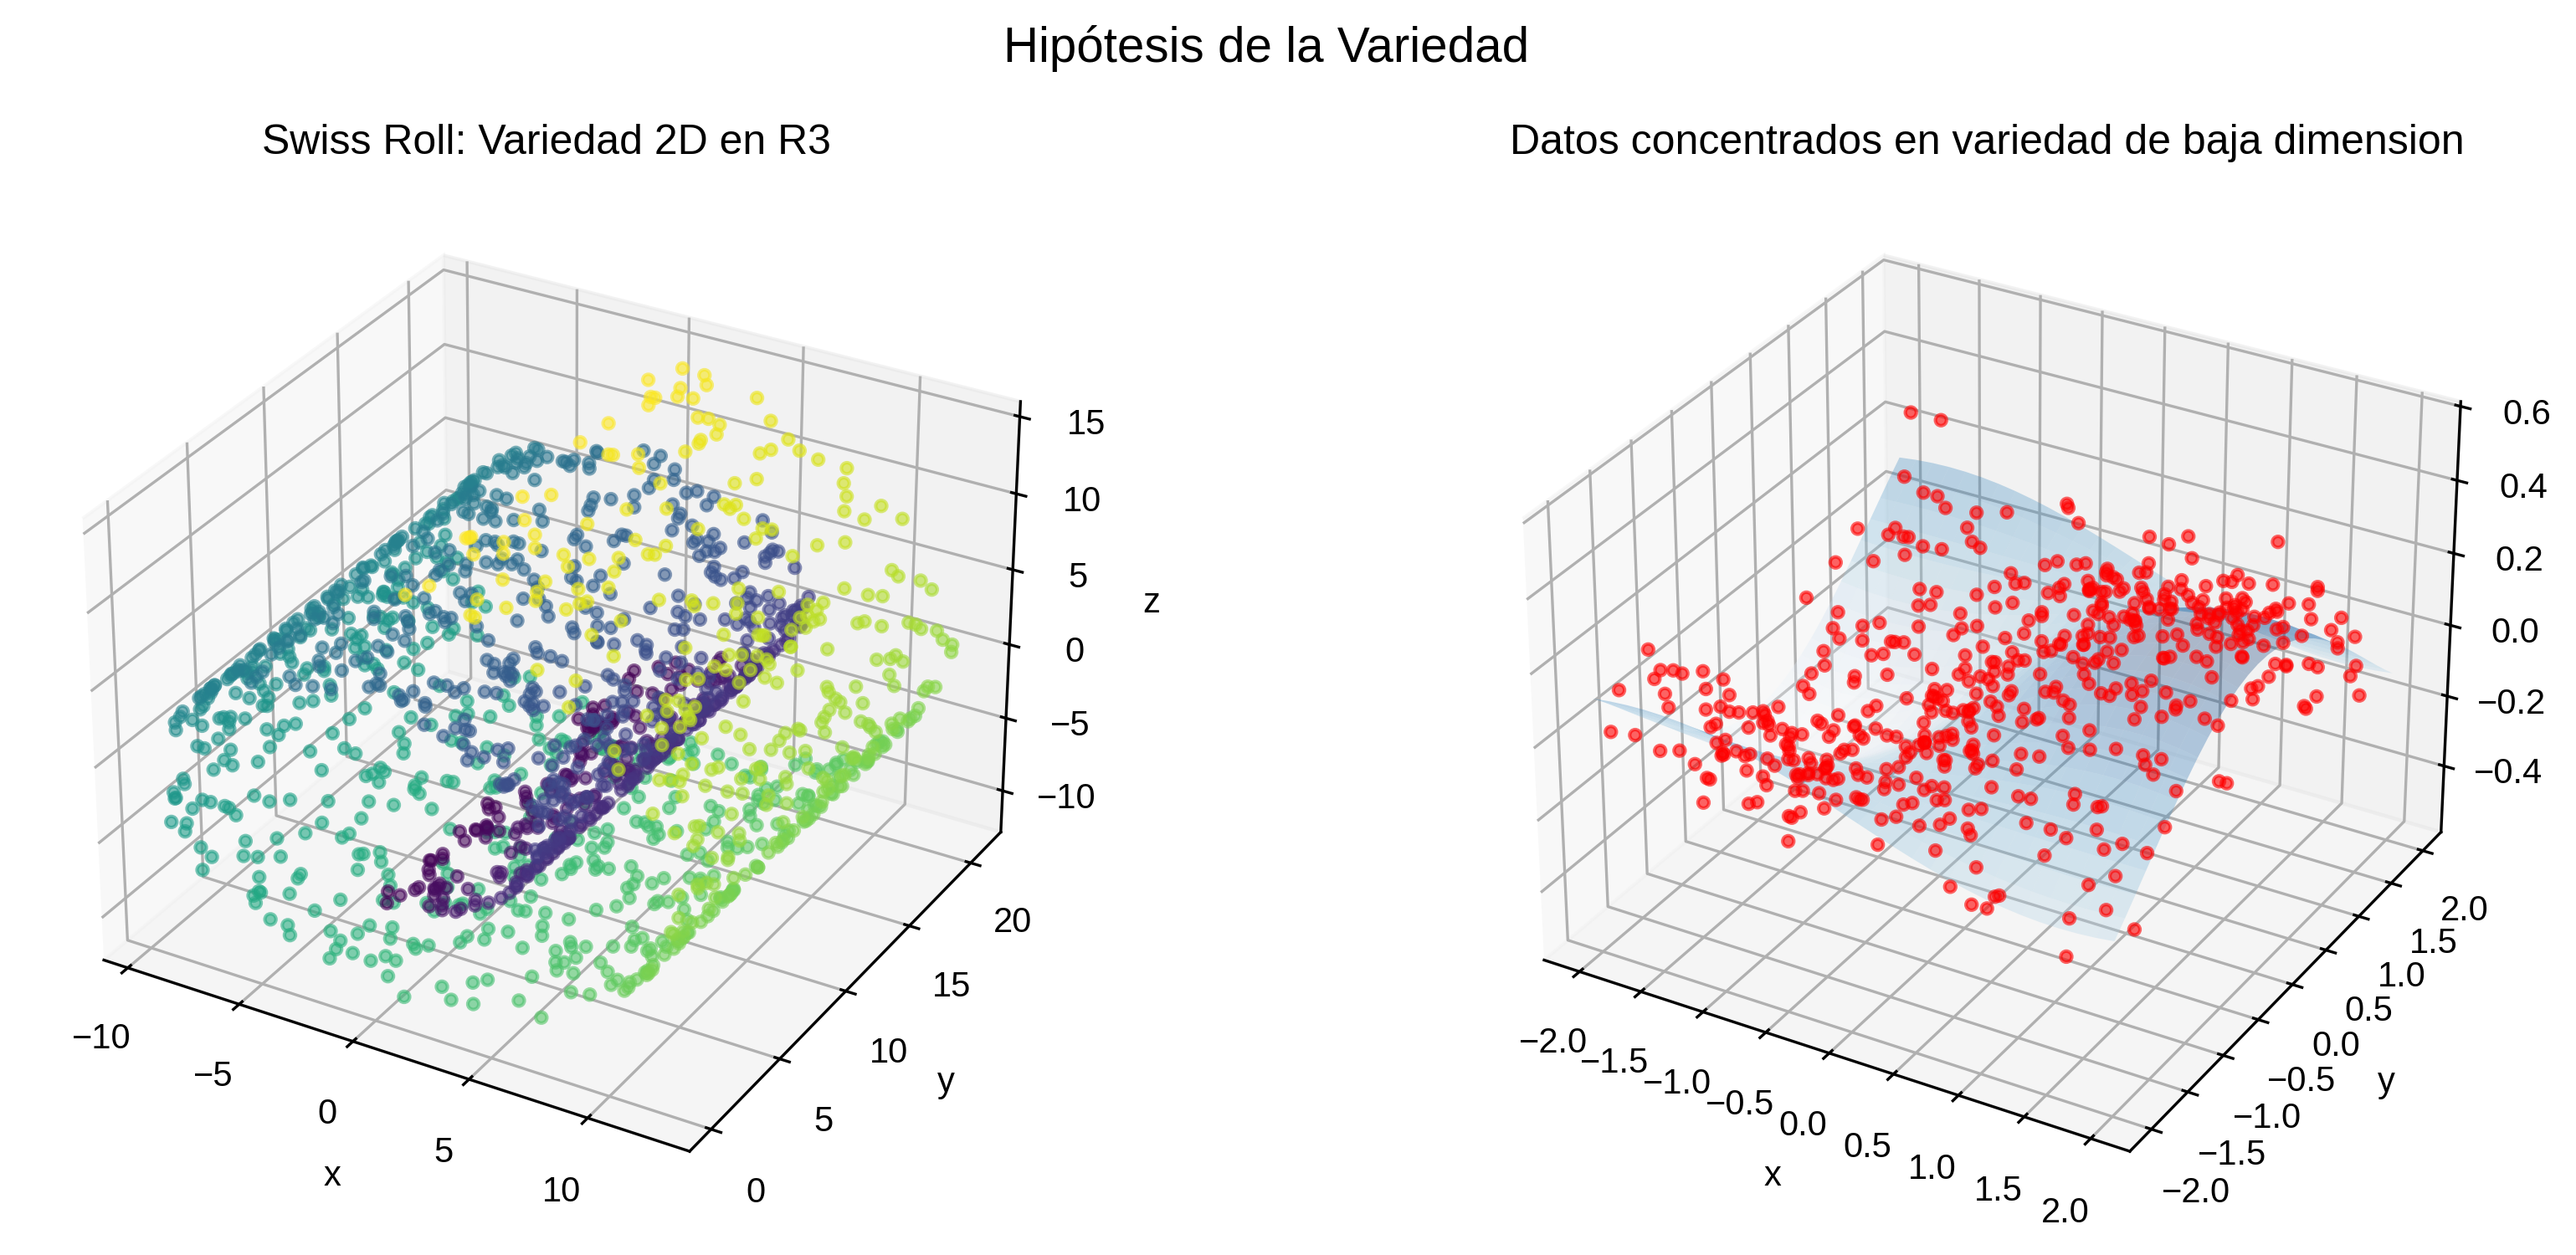
\includegraphics[width=0.9\textwidth]{images/manifold_hypothesis.png}
\caption[Manifold hypothesis]{Illustration of the manifold hypothesis. Left: the torus $\mathbb{T}^2$ as a two-dimensional manifold embedded in $\mathbb{R}^3$. Right: hyperbolic paraboloid (saddle) with data distributed over the surface, illustrating how high-dimensional data concentrates on low-dimensional manifolds.}
\label{fig:manifold_hypothesis}
\end{figure}

\begin{hypothesis}[Manifold hypothesis]\label{hyp:hipotesis_variedad_gdl}
High-dimensional data in real applications typically lies near a manifold $\mathcal{M}$ of intrinsic dimension $m \ll d$ immersed in $\mathbb{R}^d$. Formally, there exists a differentiable manifold $\mathcal{M}$ such that the probability density of the data $p(\mathbf{x})$ concentrates in a neighborhood of $\mathcal{M}$:
\[
p(\mathbf{x}) \approx 0 \quad \text{for } \mathbf{x} \notin \mathcal{U}_\epsilon(\mathcal{M})
\]
where $\mathcal{U}_\epsilon(\mathcal{M})$ is an $\epsilon$-tubular neighborhood of $\mathcal{M}$.
\end{hypothesis}

This hypothesis is not merely speculative: it has a solid theoretical foundation and abundant empirical evidence. The following fundamental results characterize the structure of manifolds in high-dimensional spaces.

\begin{theorem}[Whitney Embedding Theorem]\label{thm:whitney_embedding}
Let $\mathcal{M}$ be a compact differentiable manifold of dimension $m$. Then $\mathcal{M}$ can be smoothly embedded in $\mathbb{R}^{2m+1}$ and, if $m > 1$, immersed in $\mathbb{R}^{2m-1}$.
\end{theorem}

\begin{proof}[Sketch]
The proof proceeds in two phases: first an embedding into a Euclidean space of arbitrarily large dimension is constructed, and then the dimension is iteratively reduced until reaching $\mathbb{R}^{2m+1}$.

\textbf{Step 1: Immersion in high dimension.}
By compactness, $\mathcal{M}$ admits a finite atlas $\{(U_i, \phi_i)\}_{i=1}^N$. Let $\{\rho_i\}_{i=1}^N$ be a partition of unity subordinate to this cover, that is, smooth functions $\rho_i: \mathcal{M} \to [0,1]$ with $\operatorname{supp}(\rho_i) \subset U_i$ and $\sum_i \rho_i \equiv 1$. We define $F: \mathcal{M} \to \mathbb{R}^{N(m+1)}$ by:
\[
F(p) = \bigl(\rho_1(p)\phi_1(p), \ldots, \rho_N(p)\phi_N(p), \rho_1(p), \ldots, \rho_N(p)\bigr)
\]
where $\rho_i(p)\phi_i(p) = 0$ when $p \notin U_i$.

\textbf{Step 2: $F$ is an embedding.}
The map $F$ is smooth, being a composition of smooth functions. It is injective: if $F(p) = F(q)$, the last $N$ components give $\rho_i(p) = \rho_i(q)$ for all $i$; choosing $i$ with $\rho_i(p) > 0$, the first components give $\rho_i(p)\phi_i(p) = \rho_i(q)\phi_i(q)$, whence $\phi_i(p) = \phi_i(q)$ and therefore $p = q$. To see that $dF_p$ (\autoref{def:diferencial_aplicacion_suave}) is injective, we fix $i$ with $\rho_i(p) > 0$: the corresponding block of the differential contains $\rho_i(p) \cdot d(\phi_i)_p$, which has rank $m$ since $\phi_i$ is a local diffeomorphism. Since $\mathcal{M}$ is compact, by \autoref{rem:compacta_inmersion_embebimiento} this injective immersion is an embedding.

\textbf{Step 3: Dimension reduction.}
One iteratively projects from $\mathbb{R}^k$ to $\mathbb{R}^{k-1}$ by choosing a direction $\mathbf{v} \in S^{k-1}$ and projecting orthogonally onto $\mathbf{v}^\perp \cong \mathbb{R}^{k-1}$. The projection $\pi_\mathbf{v}$ restricted to $F(\mathcal{M})$ fails to be an embedding only if $\mathbf{v}$ is tangent to $F(\mathcal{M})$ (loss of injectivity of the differential) or if $\mathbf{v}$ is a secant direction, that is, $\mathbf{v} \propto F(p) - F(q)$ for some pair $p \neq q$ (loss of global injectivity). The set of tangent directions has dimension $\leq 2m - 1$ in $S^{k-1}$ (image of the unit tangent bundle, of dimension $2m-1$) and that of secant directions has dimension $\leq 2m$ (image of $\mathcal{M} \times \mathcal{M} \setminus \Delta$, of dimension $2m$). By Sard's Theorem (\autoref{thm:sard}, see \autoref{sec:sard} of Appendix~\ref{ch:teoremas_complementarios}), the set of critical values of the maps that parameterize these directions has measure zero in $S^{k-1}$. Since $\dim S^{k-1} = k - 1 > 2m$ when $k > 2m + 1$, there exist ``good'' directions and the projection preserves the embedding. Iterating, one obtains an embedding in $\mathbb{R}^{2m+1}$.

\textbf{Strong version.}
The improvement from $\mathbb{R}^{2m+1}$ to $\mathbb{R}^{2m}$ requires additional techniques (the ``Whitney trick'') to eliminate residual self-intersections; see \citep[Chapter 6]{lee2012introduction}.
\end{proof}

Whitney's theorem guarantees that any compact $m$-dimensional manifold can be faithfully represented in $\mathbb{R}^{2m+1}$. This theoretically justifies why high-dimensional representations work: if the data really resides on a manifold of dimension $m$, then embeddings in $\mathbb{R}^{2m+1}$ or higher are sufficient to capture all of its geometric structure. However, the theorem does not provide an efficient constructive algorithm, which motivates the use of dimensionality reduction techniques such as variational autoencoders and \gls{GDL}.

\begin{definition}[Reach of a manifold]\label{def:reach}
Let $\mathcal{M} \subset \mathbb{R}^d$ be an embedded closed manifold. The \textit{reach} of $\mathcal{M}$, denoted $\tau(\mathcal{M})$, is the maximum value of $r > 0$ such that any point $\mathbf{x} \in \mathbb{R}^d$ with $d(\mathbf{x}, \mathcal{M}) < r$ has a unique projection onto $\mathcal{M}$.
\end{definition}

The reach characterizes how ``regular'' the geometry of the manifold is: large reach indicates smooth curvature and absence of self-proximity, while small reach indicates complex geometry with regions of high curvature.

\begin{proposition}[Sample complexity on manifolds]\label{prop:complejidad_muestral_variedades}
Let $\mathcal{M}$ be a compact Riemannian manifold (\autoref{def:espacio_compacto}) of dimension $m$, with reach $\tau > 0$ and sectional curvature bounded in absolute value by $\kappa$. Then, to uniformly approximate an $L$-Lipschitz function $f: \mathcal{M} \to \mathbb{R}$ with error $\epsilon$ from samples, the following number of samples is required:
\[
N = \Omega\left(\left(\frac{1}{\epsilon}\right)^m \cdot \operatorname{poly}(\tau^{-1}, \kappa)\right)
\]
\citep{niyogi2008finding}.
\end{proposition}

For a sketch of the proof based on covering numbers and volume comparison, see \autoref{sec:complejidad_muestral} of Appendix~\ref{ch:teoremas_complementarios}.

This proposition reveals that the sample complexity depends on the \textbf{intrinsic dimension} $m$ of the manifold, not on the ambient dimension $d$. This is the ``blessing of dimensionality'': if the high-dimensional data really resides on a low-dimensional manifold, then the number of samples needed for learning is exponentially smaller than what the ambient dimension would suggest. This explains why neural networks work effectively in high-dimensional spaces such as images ($d \sim 10^6$) or text sequences ($d \sim 10^4$): the effective intrinsic dimension $m$ is much smaller.

\paragraph{Examples of manifolds in real data}

The manifold hypothesis is not abstract: it manifests concretely in real application domains:

\begin{itemize}
    \item \textbf{Natural images}: Although a $256 \times 256$ RGB image is formally a vector in $\mathbb{R}^{196608}$, natural images do not uniformly fill this space. They concentrate on a manifold of estimated dimension between 10 and 100, determined by semantic structures (objects, textures, illumination) and natural statistics.

    \item \textbf{Configurations of articulated robots}: A robotic arm with $n$ joints has configurations that reside in the product of circles $(S^1)^n$, a compact manifold of dimension $n$. Although we can represent each configuration as a vector of angles in $\mathbb{R}^n$, the intrinsic topology is non-Euclidean: the angle $2\pi$ is identical to the angle $0$.

    \item \textbf{Brain diffusion MRI data}: The neural fibers in diffusion magnetic resonance imaging live in the tangent bundle of the brain manifold. At each voxel, the diffusion direction is a vector tangent to the cortical surface, not an arbitrary vector in $\mathbb{R}^3$.
\end{itemize}

\subsection{Non-Euclidean Spaces}\label{subsec:espacios_no_euclidianos}

The manifold hypothesis establishes that data resides on low-dimensional manifolds, but these manifolds are, in general, non-Euclidean spaces whose intrinsic geometry differs from the Euclidean one. Non-Euclidean spaces therefore provide the concrete geometric framework for modeling data manifolds: each type of curvature and topology gives rise to distinct geometric operations that, as we will see, determine the appropriate neural architecture. Notably, all the geometries we will study in this section (spheres, projective spaces, Grassmann manifolds, hyperbolic spaces) share a common algebraic structure that allows building equivariant architectures in a unified way; this structure is formalized in \autoref{subsec:espacios_homogeneos}.

\paragraph{Origin of non-Euclidean geometries}

Non-Euclidean geometries arise from modifying Euclid's fifth postulate. In the language of modern differential geometry (\autoref{subsec:variedades_riemannianas}), this modification corresponds to considering Riemannian manifolds with nonzero curvature:

\begin{itemize}
    \item \textbf{Hyperbolic geometry} \citep{gray2007worlds}: Through a point external to a line pass \textit{infinitely many} parallel lines. Developed independently by Lobachevsky and Bolyai around 1830, it corresponds to manifolds with constant sectional curvature $K < 0$. The canonical model is the hyperbolic space $\mathbb{H}^n$ with $K = -1$.
    \item \textbf{Elliptic/spherical geometry} \citep{riemann1854hypothesen}: Through a point external to a line passes \textit{no} parallel line (all geodesics intersect). Formalized by Riemann in 1854, it corresponds to manifolds with constant sectional curvature $K > 0$. The canonical model is the sphere $S^n$ with $K = +1$.
\end{itemize}

In the context of \gls{GDL}, these geometric properties (see \autoref{rem:significado_curvatura}) have direct implications for the design of neural architectures: the curvature of the domain determines how information propagates between neighboring points, since in spaces of positive curvature information converges (facilitating global aggregation), while in negative curvature the representational capacity grows exponentially with distance (facilitating hierarchical representations). Choosing the appropriate geometric space amounts, in this sense, to incorporating a geometric inductive bias into the architecture. We next examine each concrete space, presenting its formal definition, its geometric properties, and its characteristic applications.


\begin{figure}[htbp]
\centering
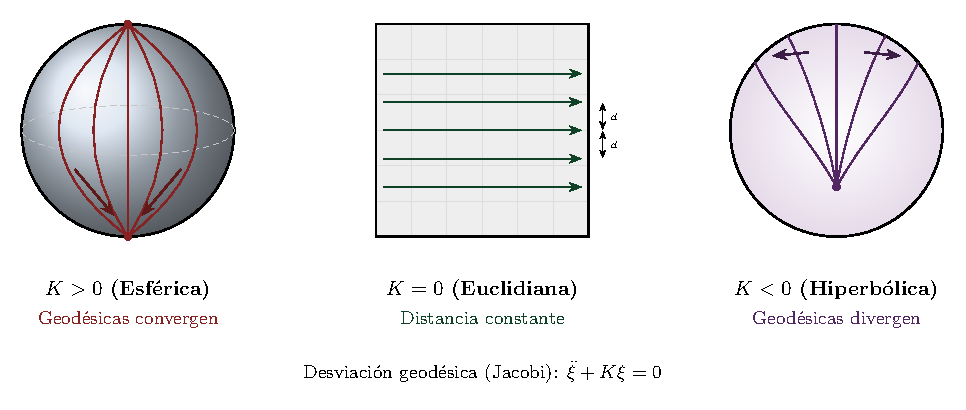
\includegraphics[width=0.85\textwidth]{images/curvature_comparison.pdf}
\caption[Comparison of geometries according to curvature]{Comparison of the three classical geometries according to the sign of the sectional curvature $K$. In positive curvature ($K > 0$), geodesics converge, facilitating the global aggregation of information. In zero curvature ($K = 0$), geodesics maintain constant distance (Euclidean geometry). In negative curvature ($K < 0$), geodesics diverge exponentially, providing greater representational capacity for hierarchical data.}
\label{fig:curvature_comparison}
\end{figure}

\paragraph{Spheres and projective spaces: directional data}

\begin{definition}[$n$-dimensional sphere]\label{def:esfera_n}
The \textit{$n$-dimensional sphere} is the manifold:
\[
S^n = \{x \in \mathbb{R}^{n+1} : \|x\| = 1\}
\]
The Riemannian metric induced by the ambient Euclidean metric has constant sectional curvature $+1$ (see \autoref{thm:curvatura_esfera} of Appendix~\ref{ch:teoremas_complementarios}).
\end{definition}

The spheres $S^{n-1} \subset \mathbb{R}^n$ are fundamental for directional data where only the orientation matters, not the magnitude, with intrinsic metric given by the angular distance:
\[
d_{S^{n-1}}(\mathbf{u}, \mathbf{v}) = \arccos(\mathbf{u}^T \mathbf{v})
\]

\textbf{Key applications}:
\begin{itemize}
    \item \textbf{Omnidirectional vision}: $360^\circ$ panoramic images naturally live on $S^2$. \glspl{SphericalCNN} \citep{cohen2018sphericalcnns} operate directly on the sphere using convolutions equivariant under $SO(3)$, avoiding the distortions of planar projections (see \autoref{subsec:spherical_cnns_so3}).

    \item \textbf{Normalized embeddings}: In metric learning, normalizing embeddings to the unit sphere $S^{d-1}$ improves generalization capacity by focusing on directionality rather than magnitude \citep{wang2017normface} (see \autoref{subsec:atencion_esfera}).

    \item \textbf{Molecular orientations}: Directions of chemical bonds and dipole moments are naturally elements of $S^2$, with rotational symmetries under $SO(3)$.

    \item \textbf{Architectural implication}: The constant positive curvature of $S^n$ implies that convolutions must replace Euclidean translations with rotations of the group $SO(n+1)$. \glspl{SphericalCNN} exploit this by defining convolution as cross-correlation over $SO(3)$, guaranteeing exact rather than approximate rotational equivariance (see \autoref{subsec:spherical_cnns_so3}).
\end{itemize}

In many applications, the data represents \textit{directions} but does not distinguish between opposite senses: a line in an image, an axis of rotation, or a principal direction in \gls{PCA}. This data does not live on the sphere $S^{n-1}$ (where $\mathbf{v}$ and $-\mathbf{v}$ are distinct points), but in the \textbf{real projective space}.

\begin{definition}[Real Projective Space]\label{def:espacio_proyectivo}
The \textit{real projective space} $\mathbb{RP}^n$ is the space of lines passing through the origin in $\mathbb{R}^{n+1}$, that is, the quotient of $S^n$ by the antipodal identification $x \sim -x$:
\[
\mathbb{RP}^n = S^n / \{\pm 1\}
\]
As a manifold, $\dim \mathbb{RP}^n = n$, since the antipodal projection $\pi: S^n \to \mathbb{RP}^n$ is a double cover (local diffeomorphism). The space $\mathbb{RP}^n$ is compact and connected (continuous image of $S^n$), but not simply connected: its fundamental group is $\pi_1(\mathbb{RP}^n) \cong \mathbb{Z}/2\mathbb{Z}$, with $S^n$ ($n \geq 2$) being its universal cover.

Concrete cases: $\mathbb{RP}^1 \cong S^1$ (the circle, since the identification of diametrically opposite points on $S^1$ again produces a circle); $\mathbb{RP}^2$ is the first non-orientable closed manifold (the Möbius band is an open subset of $\mathbb{RP}^2$).
\end{definition}

The canonical metric of $\mathbb{RP}^n$ is inherited from the round metric of $S^n$ through the antipodal projection, which is a local isometry (Riemannian cover):
\[
d_{\mathbb{RP}^n}([x], [y]) = \arccos(|x^T y|)
\]
The absolute value in the argument of the arccosine distinguishes this metric from the spherical one $d_{S^n}(x,y) = \arccos(x^T y)$, reflecting that $[x] = [-x]$ in $\mathbb{RP}^n$. Since $\pi: S^n \to \mathbb{RP}^n$ is a Riemannian cover (local isometry), the sectional curvature of $\mathbb{RP}^n$ is constant $+1$, equal to that of $S^n$; the geometric differences between the two spaces are purely global (orientability, fundamental group).

\textbf{Key applications} of projective spaces:
\begin{itemize}
    \item \textbf{Computer vision}: Lines and edges in images are elements of $\mathbb{RP}^2$, since a line has no ``preferred direction''. Networks that process this data must be invariant under the antipodal identification $\mathbf{v} \sim -\mathbf{v}$; projective geometric algebra provides a natural framework for encoding this symmetry \citep{dehaan2024euclideanprojectiveconformalchoosing}.

    \item \textbf{Principal component analysis}: The principal axes of \gls{PCA} are unsigned directions, elements of $\mathbb{RP}^{n-1}$. Optimization methods over $\mathbb{RP}^{n-1}$ require Riemannian rather than Euclidean gradients, since the antipodal identification turns the space into a nontrivial manifold.

    \item \textbf{Architectural implication}: The quotient structure $\mathbb{RP}^{n-1} = S^{n-1}/\mathbb{Z}_2$ implies that the neural layers must be equivariant under the antipodal action. A projective layer can be constructed by taking a spherical layer and symmetrizing: $f([x]) = g(x) + g(-x)$. As a homogeneous space, $\mathbb{RP}^{n-1} \cong O(n)/(O(n-1) \times \mathbb{Z}_2)$ (\autoref{prop:proyectivo_cociente}), and this representation guides the construction of equivariant networks over the projective space.
\end{itemize}

\begin{definition}[Grassmann manifold]\label{def:variedad_grassmann}
The \textit{Grassmann manifold} $Gr(k,n)$ is the space of all $k$-dimensional subspaces of $\mathbb{R}^n$. It is a compact manifold of dimension $\dim Gr(k,n) = k(n-k)$. Each point of $Gr(k,n)$ can be uniquely represented by the orthogonal projection matrix $P \in \mathbb{R}^{n \times n}$ onto the corresponding subspace, characterized by:
\[
P^2 = P, \qquad P^T = P, \qquad \operatorname{tr}(P) = k
\]
The real projective space is the special case $\mathbb{RP}^{n-1} = Gr(1,n)$ (lines through the origin). As concrete cases: $Gr(1,3) = \mathbb{RP}^2$ parameterizes the lines in $\mathbb{R}^3$, and $Gr(2,4)$ (planes in $\mathbb{R}^4$) has dimension $2 \cdot 2 = 4$.
\end{definition}

The natural metric of $Gr(k,n)$ is based on the \textit{principal angles} between subspaces. Given $U, V \in Gr(k,n)$, the principal angles $\theta_1, \ldots, \theta_k \in [0, \pi/2]$ are the angles between the most aligned pairs of vectors of $U$ and $V$ (defined recursively as $\cos \theta_i = \max_{u \in U, v \in V} u^T v$ subject to orthonormality with the previous pairs). The geodesic distance is:
\[
d_{Gr}(U, V) = \sqrt{\sum_{i=1}^{k} \theta_i^2}
\]
When $k = 1$, this metric reduces to the Fubini-Study metric over $\mathbb{RP}^{n-1}$. The Grassmann manifold also possesses a natural symmetry $Gr(k,n) \cong Gr(n-k,n)$ (duality by orthogonal complement: to each subspace $V$ corresponds $V^\perp$), which in dimension $k(n-k) = (n-k)k$ is reflected in the equality of dimensions.

Grassmann manifolds are relevant for data that represents linear subspaces rather than points. Since subspaces do not admit standard addition or scaling, the neural network operations must respect the curved geometry of $Gr(k,n)$.

\textbf{Key applications}:
\begin{itemize}
    \item \textbf{Action recognition in video}: Sequences of frames are modeled as subspaces of $\mathbb{R}^n$, and classification operates over $Gr(k,n)$ with geodesic metrics between subspaces. The GrassmannNet of \citet{huang2017grassmann} define layers that operate through projections and re-orthogonalizations that preserve the subspace structure.

    \item \textbf{Local principal component analysis}: In many vision tasks, the local descriptors of an image generate subspaces whose comparison requires the Grassmann metric, not the Euclidean one. The geodesic distance based on principal angles provides a similarity measure intrinsic to the space of subspaces.

    \item \textbf{Architectural implication}: The standard operations (addition, scaling) do not preserve the subspace structure in $Gr(k,n)$, so neural networks must redefine their basic operations: propagation uses exponential and logarithmic maps between the tangent space and the manifold, and linear layers are replaced by transformations that preserve membership in $Gr(k,n)$ \citep{huang2017grassmann}. As a homogeneous space, $Gr(k,n) \cong O(n)/(O(k) \times O(n-k))$ (\autoref{prop:grassmann_stiefel_cociente}), which allows deriving the network operations from the representation theory of the orthogonal group.
\end{itemize}


\paragraph{Hyperbolic spaces: hierarchical data}

\begin{definition}[Hyperbolic Space]\label{def:espacio_hiperbolico}
The \textit{hyperbolic space} $\mathbb{H}^n$ is the unique simply connected space of constant sectional curvature $-1$ (the proof that $K = -1$ is presented in \autoref{thm:curvatura_hiperbolico} of Appendix~\ref{ch:teoremas_complementarios}). Geometrically, it is the $n$-dimensional analogue of the Lobachevsky-Bolyai hyperbolic plane.
\end{definition}

\textbf{Models of hyperbolic space.}\label{rem:modelos_hiperbolico} There exist several isometric models of $\mathbb{H}^n$:
\begin{itemize}
    \item \textbf{Poincaré disk model}: $\mathbb{D}^n = \{x \in \mathbb{R}^n : \|x\| < 1\}$
          with metric $ds^2 = \frac{4}{(1 - \|\mathbf{x}\|^2)^2} \sum_{i=1}^n (dx^i)^2$
    \item \textbf{Upper half-plane model}: $\mathbb{H}^2 = \{z \in \mathbb{C} : \Im(z) > 0\}$
          with metric $ds^2 = \frac{dx^2 + dy^2}{y^2}$
    \item \textbf{Hyperboloid model}: Surface $x_0^2 - x_1^2 - \cdots - x_n^2 = 1$ in $\mathbb{R}^{n+1}$
\end{itemize}

These three models are isometric as Riemannian manifolds; the explicit proof of the isometries between them (through stereographic projection and the Cayley transform) is presented in \autoref{sec:isometrias_hiperbolico} of Appendix~\ref{ch:teoremas_complementarios}.

The hyperbolic spaces $\mathbb{H}^n$ possess constant negative curvature, which confers on them a distinctive geometric property: the volume of geodesic balls grows exponentially with the radius. This characteristic makes them ideal for representing hierarchical and tree-structured data.

\textbf{Key applications}:
\begin{itemize}
    \item \textbf{Knowledge graphs and lexical semantics}: Taxonomic hierarchies (WordNet, biological ontologies) and hyperonymy (is-a) relations in natural language are embedded with less distortion in $\mathbb{H}^n$ than in $\mathbb{R}^n$ \citep{nickel2017poincare}. The required dimensionality is logarithmic rather than exponential (see Section~\ref{subsubsec:embeddings_hiperbolicos_grafos} for the mathematical justification and its connection with hyperbolic attention mechanisms).

    \item \textbf{Social networks}: Hierarchical communities in social networks exhibit a tree structure that is naturally captured in hyperbolic geometry \citep{krioukov2010hyperbolic}.
\end{itemize}

\textbf{Architectural implication}: The negative curvature of $\mathbb{H}^n$ requires redefining the basic operations of neural networks. Vector addition is replaced by \textit{Möbius addition} in the Poincaré disk model, and matrix multiplication is adapted through \textit{exponential and logarithmic maps} that transport vectors between the (Euclidean) tangent space and the (hyperbolic) manifold. The Poincaré disk model $\mathbb{D}^n$ is the most used computationally for its differentiability and compatibility with gradient-based optimization \citep{nickel2017poincare}.

\begin{figure}[htbp]
\centering
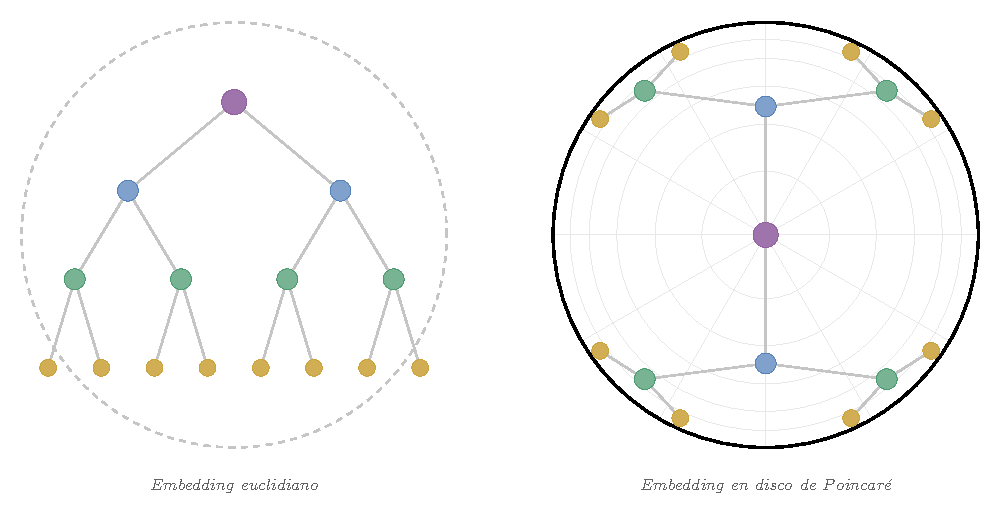
\includegraphics[width=\textwidth]{images/hyperbolic_embedding}
\caption[Hierarchical embedding in the Poincaré disk]{Embedding of a hierarchical structure in the Poincaré disk $\mathbb{D}^2$. The exponential growth of volume in hyperbolic geometry allows representing trees and hierarchies with minimal distortion, in contrast to Euclidean space where the required dimensionality grows exponentially.}
\label{fig:hyperbolic_embedding}
\end{figure}

\paragraph{Product and composite spaces: multi-structured data}

Much real-world data combines multiple types of geometry. \textbf{Product spaces} allow modeling this structural heterogeneity.

\begin{definition}[Product Manifold]\label{def:variedad_producto}
Given two Riemannian manifolds $(\mathcal{M}, g_\mathcal{M})$ and $(\mathcal{N}, g_\mathcal{N})$, the \textit{product manifold} $\mathcal{M} \times \mathcal{N}$ is the manifold whose underlying set is the Cartesian product, equipped with the \textit{product metric}:
\[
g_{(p,q)}((v_1, w_1), (v_2, w_2)) = g_{\mathcal{M},p}(v_1, v_2) + g_{\mathcal{N},q}(w_1, w_2)
\]
for $p \in \mathcal{M}$, $q \in \mathcal{N}$, $v_i \in T_p\mathcal{M}$, $w_i \in T_q\mathcal{N}$.
\end{definition}

\begin{proposition}[Properties of product manifolds]\label{prop:propiedades_producto}
The product manifold $\mathcal{M} \times \mathcal{N}$ satisfies:
\begin{enumerate}
    \item $\dim(\mathcal{M} \times \mathcal{N}) = \dim \mathcal{M} + \dim \mathcal{N}$
    \item The geodesics are products of geodesics: $\gamma(t) = (\gamma_\mathcal{M}(t), \gamma_\mathcal{N}(t))$
    \item The sectional curvatures of planes tangent to each factor are preserved
\end{enumerate}
\end{proposition}

\begin{proof}
\leavevmode
\begin{enumerate}
    \item \textbf{Dimension.} The tangent spaces satisfy $T_{(p,q)}(\mathcal{M} \times \mathcal{N}) \cong T_p\mathcal{M} \oplus T_q\mathcal{N}$, hence $\dim(\mathcal{M} \times \mathcal{N}) = \dim T_p\mathcal{M} + \dim T_q\mathcal{N} = \dim \mathcal{M} + \dim \mathcal{N}$.

    \item \textbf{Geodesics.} The product metric $g = g_\mathcal{M} + g_\mathcal{N}$ has block-diagonal structure on the tangent spaces. The geodesic equation $\nabla_{\dot\gamma}\dot\gamma = 0$ decouples into the components of each factor, since the mixed Christoffel symbols vanish. Hence $\gamma(t) = (\gamma_\mathcal{M}(t), \gamma_\mathcal{N}(t))$ is a geodesic if and only if each component is a geodesic in its factor.

    \item \textbf{Sectional curvatures.} Let $\sigma$ be a plane tangent to $\mathcal{M}$ at $(p,q)$, that is, $\sigma \subset T_p\mathcal{M} \oplus \{0\}$. The Riemann tensor of the product metric is block-diagonal (the mixed terms vanish), hence $K_{\mathcal{M}\times\mathcal{N}}(\sigma) = K_\mathcal{M}(\sigma)$. \qedhere
\end{enumerate}
\end{proof}

\begin{definition}[$n$-dimensional torus]\label{def:toro_n}
The \textit{$n$-dimensional torus} is the product of $n$ circles:
\[
T^n = \underbrace{S^1 \times S^1 \times \cdots \times S^1}_{n \text{ times}} = (\mathbb{R}/\mathbb{Z})^n
\]
The torus has zero curvature (it is flat) and admits periodic coordinates $(\theta_1, \ldots, \theta_n) \in [0, 2\pi)^n$.
\end{definition}

\textbf{Applications of product spaces:}

\begin{itemize}
    \item \textbf{Torus} $T^n = (S^1)^n$: For periodic data such as cyclic time series (seasonal climate patterns, circadian rhythms) and Fourier analysis.

    \item \textbf{Products of manifolds}: Graphs with geometric node attributes can be modeled as products $G \times \mathcal{M}$, where $G$ is the discrete structure of the graph and $\mathcal{M}$ is the space of continuous attributes.

    \item \textbf{Mixed-curvature embeddings}: Data with heterogeneous structure (partially hierarchical, partially cyclic) is represented in products $\mathbb{H}^{d_1} \times S^{d_2} \times \mathbb{R}^{d_3}$, where each component captures a different geometric aspect of the data. The dimensionality of each factor is learned automatically \citep{bronstein2017geometricdeeplearning}.
\end{itemize}

\paragraph{Graphs as discrete geometry}

Graphs $G = (V, E)$ represent a special case of \textit{discrete} non-Euclidean geometry. As developed extensively in \autoref{sec:grafos_discretizacion}, graphs provide a more flexible representation than Euclidean spaces by capturing arbitrary connectivity without imposing rigid metrics.

\paragraph{Synthesis: geometry as inductive bias}

The choice of the geometric space is not a mere representation detail: it constitutes a fundamental \textit{inductive bias} that determines the appropriate neural architecture. Each geometry imposes specific restrictions on the admissible operations:

\begin{table}[htbp]
\centering
\small
\caption{Correspondence between geometries, inductive biases, and operations in GDL.}
\label{tab:geometria_sesgo_operacion}
\begin{tabular}{@{}lll@{}}
    \toprule
    \textbf{Geometry} & \textbf{Inductive bias} & \textbf{GDL operation} \\
    \midrule
    $\mathbb{R}^n$ (Euclidean) & Translational symmetry & Standard convolution \\
    $S^n$ (spherical, $K>0$) & Rotational symmetry & Convolution over $SO(n{+}1)$ \\
    $\mathbb{H}^n$ (hyperbolic, $K<0$) & Exponential hierarchy & Möbius addition, exp/log maps \\
    $Gr(k,n)$ (Grassmann) & Data as subspaces & Geodesic metrics in $Gr$ \\
    $\mathcal{M} \times \mathcal{N}$ (product) & Heterogeneous structure & Component-wise operations \\
    Graphs & Discrete connectivity & Message passing \\
    \bottomrule
\end{tabular}
\end{table}

This correspondence between geometry and architecture is the central organizing principle of \gls{GDL}: the symmetries of the geometric domain determine the equivariance constraints that the neural network must satisfy. Notably, all the spaces presented in this section admit a unified description as homogeneous spaces $G/H$, as formalized and demonstrated in \autoref{subsec:espacios_homogeneos}; the geometric interpretation of each decomposition (how $G$ and $H$ determine curvature, compactness, and volume growth) is detailed alongside each proposition in \autoref{subsec:espacios_homogeneos}. The algebraic foundations for formalizing these symmetries are developed in \autoref{sec:grupos_simetrias}, and the complete table with specific architectures and references is presented in \autoref{rem:espacios_homogeneos_arquitecturas}.
